\documentclass[UTF8,a4paper,11pt,fontset=windows]{ctexart}
\usepackage[margin=21mm,top=23mm,bottom=22mm,headheight=15pt]{geometry}
\usepackage{amsmath,amssymb,graphicx,booktabs,tabularx,array,longtable,float,needspace}
\graphicspath{{../}}
\usepackage[numbers,sort&compress]{natbib}
\usepackage{xcolor,fancyhdr,lastpage}
\usepackage[unicode,colorlinks=true,linkcolor=black,citecolor=black,urlcolor=blue!45!black,bookmarksnumbered=true]{hyperref}
\renewcommand*{\HyperDestNameFilter}[1]{zh.#1}
\newcolumntype{P}[1]{>{\raggedright\arraybackslash}p{#1}}
\newcolumntype{Y}{>{\raggedright\arraybackslash}X}
\newcolumntype{L}{>{\raggedright\arraybackslash}X}
\newcommand{\OAL}{对象-保障-生命周期（OAL）}
\newcommand{\CDUTP}{跨域无人系统信任配置规范（CDUTP）}
\newcommand{\hl}[1]{#1}
\providecommand{\natexlab}[1]{#1}
\providecommand{\bibinfo}[2]{#2}
\providecommand{\bibfield}[2]{#2}
\providecommand{\href}[2]{#2}
\renewcommand{\arraystretch}{1.25}
\setlength{\tabcolsep}{4pt}
\setlength{\parskip}{3pt}
\setlength{\parindent}{2em}
\setlength{\emergencystretch}{2em}
\linespread{1.20}
\ctexset{section={format=\Large\bfseries,beforeskip=16pt,afterskip=8pt},
subsection={format=\large\bfseries,beforeskip=12pt,afterskip=6pt}}
\pagestyle{fancy}
\fancyhf{}
\fancyhead[L]{\small 发表前内部审批}
\fancyhead[R]{\small 中文全文译稿}
\fancyfoot[C]{\small \thepage}
\hypersetup{pdftitle={空中-水面-水下无人系统中的区块链辅助任务信任：综述与概念框架（中文全文译稿）},
pdfauthor={Shaowei Liu; Jing Wu; Tanren Liu; Shengqiang He; Yakun Ren; Chengnian Long}}
\begin{document}
\setcounter{page}{32}
\begin{center}
{\small 公司内部发表前审批用}\par\vspace{7pt}
{\LARGE\bfseries 空中-水面-水下无人系统中的区块链辅助任务信任：\\[3pt]综述与概念框架}\par\vspace{8pt}
{\large 中文全文翻译}\par\vspace{9pt}
Shaowei Liu\textsuperscript{1,2}，Jing Wu\textsuperscript{1}，Tanren Liu\textsuperscript{3}，Shengqiang He\textsuperscript{3}，Yakun Ren\textsuperscript{3}，Chengnian Long\textsuperscript{1,*}
\end{center}
\begingroup\small\noindent
\textsuperscript{1} 上海交通大学，School of Automation and Intelligent Sensing，中国上海市东川路 800 号，200240；liusw1994@sjtu.edu.cn（S.L.）；jingwu@sjtu.edu.cn（J.W.）\\
\textsuperscript{2} 江苏自动化研究所，中国江苏省连云港市圣湖路 18 号，222061。\\
\textsuperscript{3} 顺丰科技有限公司（SF Technology Co., Ltd.），中国广东省深圳市南山区科技南一路 TK Chuangzhi Tiandi 大厦 B 座，518057；tanrenliu@sf-express.com（T.L.）；heshengqiang@sf-express.com（S.H.）；yakunren@sf-express.com（Y.R.）。\\
* 通讯作者：longcn@sjtu.edu.cn。\par
\medskip\noindent 学术编辑：Maurizio Talamo。收稿：2026 年 9 月 30 日；修回：2026 年 10 月 28 日；接受：2026 年 10 月 31 日。\par
\medskip\noindent 译稿说明：本译稿对应前附的 2026 年 11 月 2 日作者校正英文稿，供公司内部发表前审批。章节、公式、图表及引文编号与英文稿对应；图片保留英文原图，图题译为中文；人名、标准编号、软件名称及参考文献原始书目信息保留，参考文献另附中文题名。\par\endgroup
\vspace{8pt}
\noindent\textbf{摘要：}空中-水面-水下任务将异构无人平台、间歇性链路和多个管理域连接起来。可靠的决策必须将物理观测、受保护的记录、共享权限以及用途适合性联系起来。本结构化叙述性综述通过 89 条限定范围的主张记录，将对象-保障-生命周期（Object--Assurance--Lifecycle，OAL）框架应用于 39 项经过全文检查的机制研究。比较性综合区分了发送者认证与观测有效性、平台完整性与任务适用性，以及复制状态恢复与任务数据失效处理。按领域分层的分析和敏感性分析揭示了纳入选择与编码选择对覆盖图谱的影响。依赖图识别受输入或权限变化影响的数据产品，情境-时间-图（CTG）循环则组织对这些产品的重新评估。分区-撤销-协调案例明确了联盟角色、面向 Fabric 的应用模式、资源受限条件下的验证，以及声学链路的载荷预算。合成事件回放验证了签名、包含证明、时间规则和授权规则。在规则一致的条件下，具备策略验证能力的见证日志产生了相同的决策。因此，账本的价值取决于共同治理需求及实现成本。任务的故障与通信要求指导共识选择；提出的测试在匹配条件下比较决策质量与恢复能力。本综述将机制证据与跨域任务决策的明确组合要求联系起来。

\noindent\textbf{关键词：}任务信任；无人系统；UAV-USV-UUV 协作；区块链；数据溯源；远程证明；零信任；海事自主系统

\section{引言}

空中-水面-水下任务将无人机（UAV）、无人水面艇（USV）和无人水下航行器（UUV）结合起来，用于观测、检查、搜索和环境监测。它们在机动性与感知能力上的互补，使任务在无线电与声学链路、网关、处理服务和管理主体之间形成依赖关系\citep{li2023survey,wei20233u,pang2026cooperative}。无人机及海洋系统综述将机动性、有限能源、间歇通信、定位不确定性和恢复困难列为运行约束\citep{hayat2016survey,shakhatreh2019unmanned,bae2023survey,gonzlezgarca2020autonomous}。任务决策必须综合在这些不同条件下生成的证据。

这形成了\emph{任务信任缺口}。认证确立主体的身份；内容哈希绑定字节；复制共识则在某种故障模型下建立一致性。依赖证据作出的决策还需要证明：观测在物理上可信、时效性足够，并且适合其预期后果。带签名的声呐报告可能不准确，真实图像可能已经过时，排序正确的记录也可能来自被俘获的设备。无人机和水下安全研究描述了相应的欺骗、干扰、俘获、路由攻击和数据操纵威胁\citep{mekdad2023survey,wang2025survey,hadi2023comprehensive,jiang2019securing,yisa2021security}。将这些控制措施与数据产品的最终用途联系起来，需要明确的主张语义。

区块链方案涉及集群认证、数据采集、成员资格、溯源和审计\citep{han2022identity,tan2022blockchain,karmakar2024blockchain,islam2019bus}。无人机与海事应用综述描述了协调与共享的机会\citep{hafeez2023blockchain,alladi2020applications,mehta2020blockchain,farah2024survey,li2021survey}。其价值取决于哪些参与方必须共同治理状态、必须容忍哪些故障，以及经过认证的数据库或独立见证日志是否已经能够满足这些要求。区块链预言机文献直接指出了外部输入问题：对已记录断言达成一致，并不能证明这些断言与物理事件相符\citep{caldarelli2020oracle,albreiki2020oracles}。

相邻领域的机制提供了互补证据。零信任提供面向特定资源的授权\citep{rose2020zero,syed2022zero}；远程证明区分设备证据、评估和依赖决策\citep{birkholz2023remote}；溯源记录生产者和转换过程\citep{w3c2013provdm,w3c2013provo}；信任推断则对声誉、不确定性和行为变化建模\citep{ahmed2019trust,aaqib2023iot,jsang2016subjective}。这些机制使用不同的词汇，评估不同的主张。它们的组合是本综述的核心议题。

所提出的\OAL{}框架，将实体、平台/设备、链路/路径和数据产品，与四个保障层及六个生命周期阶段联系起来。带类型的依赖图与情境-时间-图（CTG）循环，在将该结构应用于决策时保留共同原因、事件时间和不确定性。OAL 提供主张的组织方式；已有的推断、溯源、策略和共识机制提供实现手段。

本综述作出三项相互关联的贡献。第一，将 OAL 应用于 39 项经过全文检查的机制研究，比较互补机制所提供的证据，并检验覆盖情况对纳入选择和编码选择的敏感性。第二，通过分区-撤销-协调案例，将框架与明确的许可账本模式、可执行的策略回放和通信预算相连接。具有策略验证能力的见证日志基线揭示了两种架构产生等价决策的情形。第三，基于需求的共识选择和可证伪的研究命题，将综合结果转化为评估议程。

民用任务和公开记录的联盟场景构成本文的应用背景。

\section{综述范围与方法}\label{sec:scope}
\subsection{文献识别与选择}

本结构化叙述性综述考察无人协作、通信与安全、信任推断、溯源、证明和分布式治理。2026 年 8 月 6 日，使用 32 个英文检索式查询 OpenAlex，将发表日期下限设为 2016 年 1 月 1 日，并保留每个检索式排名最高的 25 条结果。依据 DOI 或 OpenAlex 标识符去重后，得到 571 条候选记录。检索式包括“blockchain UAV swarm”“underwater wireless sensor network trust management”“UAV USV UUV cooperative systems”“remote attestation IoT survey RATS”和“blockchain network partition finality”。通过引文追踪和定向检索，补充了更早的基础研究与官方规范。Crossref 元数据用于核对书目信息，并未作为第二个独立筛选数据库。

选择优先考虑以下英文来源：描述跨域运行约束；明确提出适用于任务边界的安全或信任机制；或提供相关标准、数据集或仿真器。重复记录以及与这些问题缺少实质联系的来源，不纳入综合分析。综述文献提供背景和引文线索；原创机制研究构成分析样本。对于声誉、分布式一致性、溯源和反馈架构，保留了 2016 年以前的基础工作。通过出版商、作者仓储和官方来源的定向检索，核查了截至 2026 年 10 月 25 日的发展。表~\ref{tab:scope} 汇总了范围和证据角色。

\subsection{全文编码与综合}\label{sec:coding}

分析样本由 39 项已检查全文的原创机制贡献组成。直接领域层包括 11 项无人机研究、3 项海事自动识别系统（AIS）研究，以及 5 项以水下应用为目标的研究。20 项可迁移研究涉及声誉、雾计算卸载、溯源、证明、访问控制、共享状态或观测评估。应用领域与实际评估环境分别记录：面向水下用途、但使用陆地数据开展的实验，仍属于代理评估。四项通用共识比较研究构成一个可识别、可移除的子集。这些有目的选择的机制支持跨保障边界比较；这种选择不用于估计整个领域中的分布比例。

参考文献共 123 条。39 项编码研究是其中的子集；其余 84 条用于支撑运行背景、概念基础、标准、相关综合研究或评估资源。表~\ref{tab:reviews} 列明编码研究组及其来源。对每项研究，提取机制主张、支撑段落、来源版本和评估范围。

编码单位为明确描述的机制主张。89 条记录中的每一条，都将一个对象与一个保障层及其得到支持的生命周期阶段关联起来。一篇论文可以贡献多项主张；每项主张只对引文段落所支持的对象-层-阶段关联进行编码。对于某个确切的对象-层-阶段组合，热图单元格只对每项研究计数一次。计数描述覆盖情况，不代表可以相加的样本量或效应量。同一论文中保障层的共现表明可能存在接口；主张之间经过验证的传递需要独立证据。

证据类型记录概念论证（L0）、分析/安全推理（L1）、仿真或已记录数据评估（L2）、已实现的原型/试验台（L3）、实体运行试验（L4），以及持续的多方运行（L5）。这些类别是相互补充的证据形式，并非有序的质量评分。证据类型对应明确的机制和已记录的评估范围；实现层面的基准测试，并不能验证其所在架构提出的每一项保障主张。离线分析现场记录数据编码为 L2；未描述运行条件的硬件原型编码为 L3。对含义不明确的部署主张，采用证据所支持的较窄类别，并在提取说明中解释。

编码采用一次提取流程并核对支撑段落；未开展独立重复编码或编码者间一致性评估。敏感性分析检验领域平衡、研究纳入、含糊的身份归属、证据类型编码、应用与数据不匹配，以及移除单项研究的影响（第~\ref{sec:sensitivity} 节）。空白单元格表示没有已编码的主张。

\begin{table}[H]\small
\caption{综合分析的范围与证据角色。}\label{tab:scope}
\begin{tabularx}{\textwidth}{LLL}\toprule
\textbf{角色} & \textbf{纳入材料} & \textbf{在综合分析中的用途}\\\midrule
运行背景 & UAV、USV、UUV、网关、岸端服务；协同控制与通信 & 任务依赖关系和部署假设\\
分析样本 & 39 项全文机制研究；89 条主张记录；两个应用分层 & OAL 覆盖、限定范围的 L0-L5 证据类型及纳入/编码敏感性\\
背景基础 & 综述、声誉与分布式系统基础、标准及治理案例 & 词汇、替代方案和设计要求\\
评估资源 & 数据集、仿真器和基准评估实践 & 候选测试；不据此推定集成任务已得到验证\\
演示案例 & 可执行的策略回放与精确的应用字节核算 & 规则一致性及示例性的设计权衡\\\bottomrule
\end{tabularx}\end{table}

\section{运行背景与信任基础}
\subsection{异构任务体系}\label{sec:coalition}

UAV 提供快速重定位、视距无线电中继和光电感知。USV 携带更多能源和较大型天线，并连接声学与无线电网络。UUV 在水下目标附近作业，但大规模传输通常依赖低速声学链路，或延迟至上浮后进行。通信综述描述了由此产生的距离、带宽、时延、能耗与对准要求之间的权衡\citep{nomikos2023survey,ali2020recent,saeed2019underwater,jahanbakht2021internet}。拓扑、时钟质量和可达性可能在一次任务内发生变化。

考虑一个民用沿岸响应联盟，由主管机构 A、科研运营方 B、通信提供方 C 和签约数据提供方 D 组成。B 运行 UUV 和 UAV；C 提供 USV 中继；A 批准任务权限；D 提供独立数据和审计服务。各组织保留自身的管理身份。本地运营方可以认证设备，却可能无权改变联盟成员资格、证据策略或撤销历史。第~\ref{sec:trace} 节和第~\ref{sec:pattern} 节使用该联盟案例，明确哪些变更需要共同批准。

USV 可以同时承担声学流量中继、数据缓存、授时和融合计算。该共享依赖点发生故障，会影响若干表面上相互独立的数据产品。端到端源签名可在经过不可信中继时保留来源完整性，但选择性扣留，以及共同的时钟或转换错误仍需考虑。图~\ref{fig:architecture} 区分了受限证据路径与岸端共享状态服务。

原始图像、声呐数据、详细遥测和证明证据以加密形式保留在链下。共享记录包含承诺、成员资格、策略/模型版本、撤销信息和审计判断。容迟转发可使用 Bundle Protocol 第 7 版，以及 BPSec 的完整性与保密服务\citep{rfc9171,rfc9172}。存储转发机制使消息得以跨接触时段保存和传递；权限到期与证据年龄策略是独立的应用规则。

\subsection{任务信任与依赖决策}

\emph{任务信任}是根据可用证据和错误后果，在特定情境下决定是否为某个明确目的依赖某个对象。\emph{可信赖性}指支撑这一决定的属性：身份、测得的端点状态、链路可用性、溯源、时效性、观测质量，以及可问责的治理。同一幅图像可能适用于总体态势感知，却不适用于避碰。

对于对象 $o$、时间 $t$、情境 $c$ 和任务用途 $m$，评估与决策具有不同的接口：
\begin{equation}\begin{aligned}
T_o(t,c,m)&=\mathcal{A}(o,\mathcal{E}_{\leq t},c,m;\theta),\\
D_{r,o}(t,c,m)&=\pi_r\!\left(T_o(t,c,m),\mathcal{C}_t,m\right).
\end{aligned}\label{eq:trust}\end{equation}
其中，$\mathcal{E}_{\leq t}$ 包含截至决策时刻收到的证据，包括观测时间和谱系。评估函数 $\mathcal{A}$ 在假设 $\theta$ 下产生针对具体主张的结果及不确定性。依赖方 $r$ 在权限、截止时间、后果与资源约束 $\mathcal{C}_t$ 下，应用策略 $\pi_r$。结果可以是允许、限制、推迟或拒绝使用。主观意见、区间、有序状态和声誉值都可以实现该接口\citep{jsang2016subjective,mui2003computational,kamvar2003eigentrust}。若赋予概率解释，则需要明确的事件定义与校准证据。

\begin{figure}[!htbp]\centering
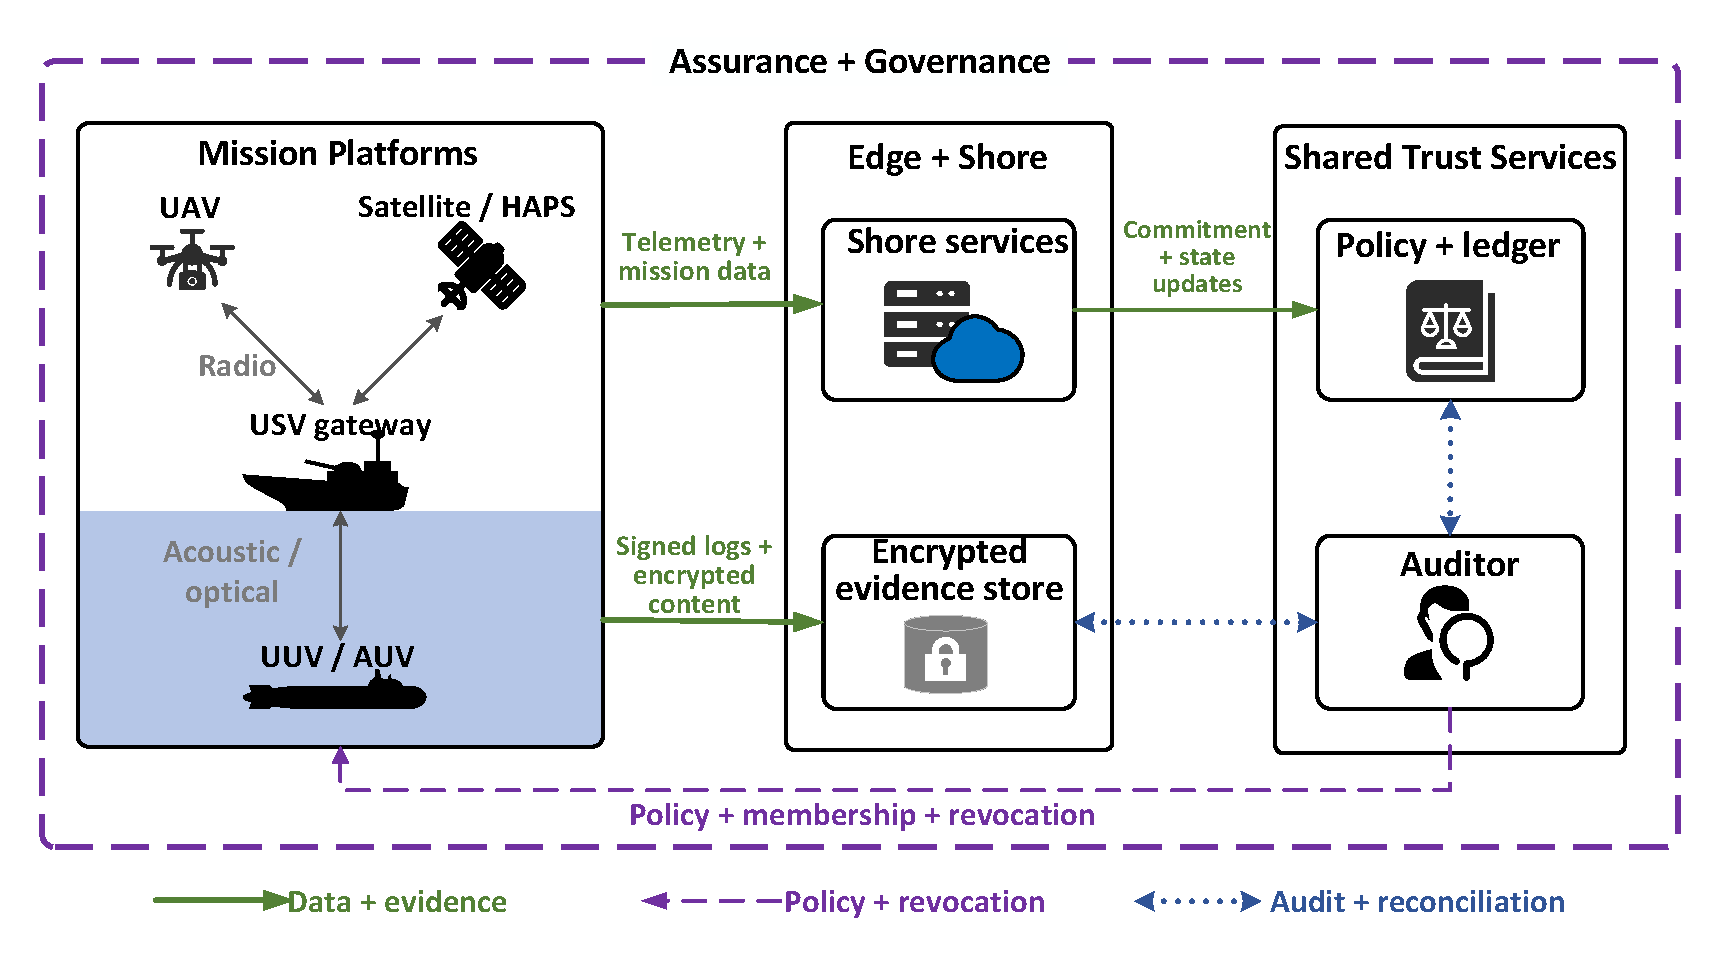
\includegraphics[width=\textwidth]{figures/figure-01-reference-architecture.pdf}
\caption{跨域参考架构。岸端组织部署对等节点与排序节点；USV 是转发/缓存依赖点。在网关分区期间，本地感知与安全控制在委托权限范围内继续运行。}\label{fig:architecture}
\end{figure}

\emph{可信数据环境}是产生、转换、共享和治理这些证据的社会技术环境。它包含主体、设备、路径、制品和问责流程。零信任提供以资源为中心的策略及执行机制\citep{rose2020zero}；OAL 则记录与任务依赖有关的附加观测、谱系、时间和后果主张。

\subsection{四类互补的保障主张}

观测有效性关注与物理世界的对应关系。承诺与溯源完整性关注受保护的字节，以及已记录的来源或转换过程。账本与治理一致性关注经过授权的共享状态转换。任务使用适合性关注特定的决策及其后果。图~\ref{fig:assurance-chain} 展示了这些不同问题及其支撑证据。

使用被盗密钥签名的伪造观测，可以通过签名验证。RATS 评估支撑限定范围的测量状态主张\citep{birkholz2023remote}，物理诊断与交叉佐证则支撑观测主张。依赖策略组合适用的结果，并明确规定要求未满足或状态未知时的响应。

\begin{figure}[!htbp]\centering
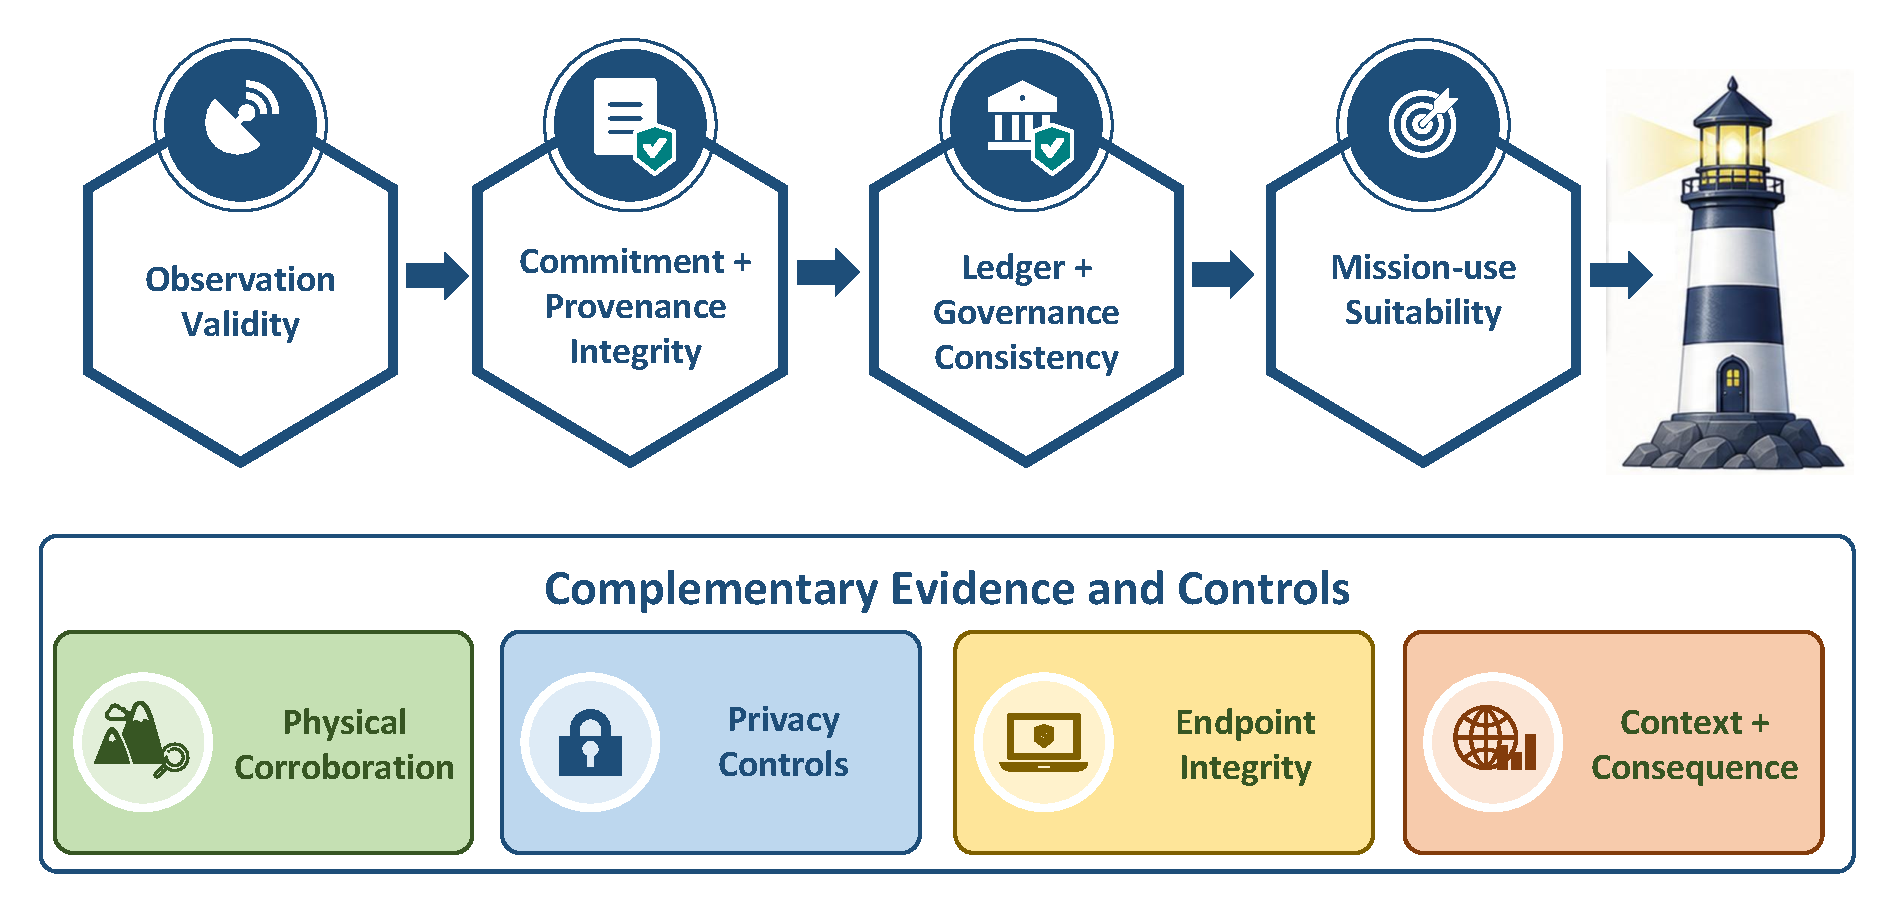
\includegraphics[width=\textwidth]{figures/figure-02-assurance-chain.pdf}
\caption{四类保障主张及其证据。图中的关系表示论证结构；实际实现可以按不同顺序执行检查。}\label{fig:assurance-chain}
\end{figure}

\section{互补的研究领域}

协同导航与编队研究建立了异构无人平台之间的交互\citep{wu2020cooperative,ke2022cooperative,xue2021distributed,liu2023formation}。这些研究中的\emph{一致性}涉及物理状态的协调。账本共识涉及在故障模型下对复制记录达成一致。OAL 通过明确的观测、转换、权限和预期用途，将它们的输出联系起来。

\subsection{安全与证据评估}

安全综述按目标和攻击机制组织欺骗、干扰、俘获、恶意路由、恶意软件和虚假数据注入\citep{yahuza2021internet,mekdad2023survey,jiang2019securing,adam2024state}。水下衰落、噪声、多普勒效应和拓扑变化，也可能造成丢失或不一致\citep{ali2020recent,jouhari2019underwater,mohsan2022towards}。因此，信任估计需要指明被评估的属性和不确定性状态：即使异常原因尚未查明，也可能有理由限制使用。

决策树和隐马尔可夫方法展示了水下信任推断\citep{jiang2020dynamic,arifeen2020hidden}。前者以初始无攻击训练期为条件，评估仿真网络行为；后者包含一个使用十个生成观测值的数值示例。这些研究在各自明确的网络与观测模型范围内支持信任推断。基于声誉的对等节点选择\citep{kamvar2003eigentrust}同样提供一种评估机制，其含义取决于服务和所观测的行为。综述分类区分直接观测、推荐、情境，以及针对声誉的攻击\citep{ahmed2019trust,aaqib2023iot,junior2021survey,liu2023survey}。

观测评估提供了另一条互补研究路径。针对 GNSS 欺骗，已有信号特征分类、网络辅助检测和记录数据验证研究\citep{shafique2021detecting,dang2022deep,semanjski2020use}。多视图意见聚合在明确假设下组合不确定观测\citep{liu2022trusted}。这些方法处理有关物理世界的证据。它们的输出成为依赖策略的输入，而该策略应明确后果和有效时间区间。

\subsection{溯源、证明与访问}

W3C PROV 对实体、活动和代理进行建模\citep{w3c2013provdm,w3c2013provo}。OAL 实体是执行行动的主体，通常映射为 PROV 代理；OAL 数据产品映射为 PROV 实体。决策溯源沿着通向组织决策或自动化决策的数据流扩展分析\citep{singh2019decision}。当事件捕获和留存记录覆盖相关转换过程时，它能够支持问责。

证明提供测得的端点状态证据。架构方案讨论了账本参与方证明和自主物联网安全\citep{hardjono2021towards,figueiredo2022arcadian}；已实现的工作则评估经过证明的通道，以及对嵌入式设备和所部署机器学习制品的双重证明\citep{ott2023universal,baciu2025secure}。RATS 区分证据、验证方评估和依赖决策\citep{birkholz2023remote}。零信任与设备基线给出授权及端点能力要求\citep{rose2020zero,syed2022zero,fagan2020iot}。在断连期间，缓存结果与委托权限分别随时间老化，因此这些边界十分关键。

\subsection{共享记录与治理}

编码样本中的无人机研究将经过认证的身份或数据采集与账本状态结合\citep{han2022identity,tan2022blockchain,karmakar2024blockchain,islam2019bus}。Fabric 提供已实现的执行-排序-验证架构\citep{androulaki2018hyperledger}；物联网平台将其应用于感知记录完整性、链下溯源和访问策略\citep{hang2019design,honarpajooh2021iot,liu2020fabric}。食品、医疗和数字孪生研究将这些模式扩展到预测、联邦学习和生命周期协调\citep{khan2020iot,rahman2020secure,suhail2022trustworthy}。表~\ref{tab:reviews} 汇总其记录的机制与评估环境，第~\ref{sec:oal} 节进行映射。

\begin{table}[H]\footnotesize
\caption{39 项编码研究及其主要证据范围。证据类型对应限定范围的主张，同一研究中的类型可以重叠。}\label{tab:reviews}
\begin{tabularx}{\textwidth}{@{}P{22mm}P{52mm}P{21mm}Y@{}}\toprule
\textbf{标识符} & \textbf{机制重点} & \textbf{证据类型} & \textbf{评估范围}\\\midrule
S01--S04 & UAV 身份/认证/采集\citep{han2022identity,tan2022blockchain,karmakar2024blockchain,islam2019bus} & L1、L2、L3 & 安全分析、仿真和已实现的组件；BUS 包含 UAV 与 IoT 硬件\\
S05--S07 & 水下信任与 P2P 声誉\citep{jiang2020dynamic,arifeen2020hidden,kamvar2003eigentrust} & L1/L2 & 网络或数值评估，以及对等节点选择仿真\\
S08--S10 & Fabric、感知记录、Hadoop 溯源\citep{androulaki2018hyperledger,hang2019design,honarpajooh2021iot} & L3 & 服务器和嵌入式设备原型；记录处理与检索\\
S11--S14 & 证明与自主 IoT 安全\citep{hardjono2021towards,ott2023universal,figueiredo2022arcadian,baciu2025secure} & L0 或 L3 & 两项架构贡献；两项已实现的证明研究\\
S15--S17 & 食品/医疗溯源与访问控制\citep{khan2020iot,rahman2020secure,liu2020fabric} & L2 和/或 L3 & 预测、联邦学习应用和受控访问策略请求\\
S18--S19 & 决策溯源与数字孪生\citep{singh2019decision,suhail2022trustworthy} & L0 & 概念性数据流和生命周期架构\\
S20--S23 & GNSS 与多视图观测评估\citep{shafique2021detecting,dang2022deep,semanjski2020use,liu2022trusted} & L1/L2 & 信号/学习实验、记录数据和聚合分析\\
S24--S26 & 视觉佐证、UAV 报告、雾计算卸载\citep{varshosaz2019spoofing,garcamagario2019security,alkhafajiy2020comitment} & L0/L2 & 记录轨迹、代理仿真，以及伙伴/资源选择建模\\
S27--S29 & 海事 AIS 溯源与消息保护\citep{maritime2022monitoring,kessler2020protected,goudossis2022secais} & L3 & 接收机/账本基准测试和两项软件保护演示\\
S30--S31、S39 & UAV 声誉、治理与路由\citep{hierarchical2023trust,yang2023trusted,barka2022towards} & L0/L2/L3/L4 & 仿真信任更新；S31 包含实体 UAV 节点实验和独立容器试验台\\
S32--S34 & 水下签密、路由与联邦学习\citep{zhang2026underwater,eetauv2025trust,tafl2026underwater} & L1/L2/L3 & 桌面密码运算、路由仿真和基于陆地数据的代理学习\\
S35--S38 & 通用共识比较研究\citep{hotstuff2019,narwhal2022,raft2014,pbft1999} & L1/L3 & 协议推理与服务器/云原型；故障模型和已测试恢复路径各异\\\bottomrule
\end{tabularx}\end{table}

预言机问题在这些应用中始终存在：账本保留被接受的断言及其溯源，而外部有效性依赖数据源和评估\citep{caldarelli2020oracle,albreiki2020oracles}。透明日志是自然的替代方案。证书透明度规范定义包含证明和一致性证明，并需要外部监控或见证来处理不一致视图\citep{rfc6962,rfc9162}。Sigstore 将签名与软件制品透明度相结合\citep{sigstore2022}。见证日志也可以承载共同授权的状态转换。因此，应评估的是所需验证与治理服务及其实现成本，而不只是是否存在哈希链。

\section{OAL 框架与文献映射}\label{sec:oal}

OAL 对\emph{判断什么}、\emph{寻求哪种主张}以及\emph{何时需要该主张}进行分类。某个机制可以支持多个单元格；某些组合可能不适用于某项任务。主张之间的依赖关系另行表示，因此分类不意味着证据相互独立。

\subsection{对象、保障层与生命周期}

\emph{实体}是可问责的主体：组织、操作人员、服务，或具有委托权限的自主代理。\emph{平台/设备}是执行功能的端点，包括无人平台、网关、传感器和承载的计算实例。当航行器行使委托权限时，可将其视为实体；测量其固件状态时，则将其视为平台。\emph{链路/路径}包括端到端路由上的物理介质、中间节点、安全关联和变化的质量。\emph{数据产品}是具有明确版本标识的观测、轨迹、地图、模型、命令、策略或审计记录。更正与转换会产生新的版本标识符。表~\ref{tab:objects} 汇总各类对象的证据和依赖问题。

\begin{table}[H]\small
\caption{OAL 对象及针对具体主张的证据。}\label{tab:objects}
\begin{tabularx}{\textwidth}{@{}P{26mm}YY@{}}\toprule
\textbf{对象} & \textbf{证据} & \textbf{依赖问题}\\\midrule
实体（E） & 凭证、角色、委托、可问责的行为 & 谁在行动，依据什么权限？\\
平台（P） & 启动/运行时测量、配置、自检、能源 & 哪个端点在执行，其测得状态如何？\\
链路/路径（L） & 认证、路由、时延、丢失、托管及介质状态 & 路径上具备什么保护与时效性？\\
数据产品（D） & 签名、内容标识、时间、谱系、不确定性、残差 & 这是哪个版本，什么证据支持其预期用途？\\\bottomrule
\end{tabularx}\end{table}

保障轴包括 O（观测有效性）、C（承诺与溯源完整性）、G（账本与治理一致性）和 M（任务使用适合性）。O 使用物理边界、校准、诊断和交叉佐证。C 通过签名与溯源绑定生产者、版本和转换断言。G 处理共同授权的成员资格、顺序、策略和恢复状态。M 应用目的、时效性、后果、不确定性和权限要求。当不需要共享状态服务时，账本特有主张不适用；等价的治理主张可以由其他服务满足。

策略、模型和参考值是带版本的数据产品；其部署实例位于平台上，其批准权限属于实体。这种处理使保障基础设施与任务观测接受相同的分析。单元格规范首先确定对象/版本及所需属性，再给出支撑证据和有效时间区间。它还指明接受规则、责任方，以及证据缺失时的响应。表~\ref{tab:lifecycle} 汇总生命周期阶段与状态转换。

\begin{table}[H]\small
\caption{生命周期阶段及相关状态转换。}\label{tab:lifecycle}
\begin{tabularx}{\textwidth}{@{}P{30mm}YY@{}}\toprule
\textbf{阶段} & \textbf{所需保障} & \textbf{保留状态示例}\\\midrule
准入（A） & 主体经过授权，端点符合接受要求 & 角色、委托、证明参考\\
感知（S） & 时间、位置和观测可信 & 产品标识、质量和采集承诺\\
传输（T） & 内容受保护，路径满足要求 & 中继/托管事件和批次根\\
融合/共享（F） & 输入、转换和访问均有明确标识 & 谱系、模型和策略版本\\
决策/行动（D） & 当前适合所指定的后果 & 决策依据和责任主体\\
恢复/审计（R） & 明确失效范围并恢复权限 & 撤销、争议和协调后的历史\\\bottomrule
\end{tabularx}\end{table}

\subsection{编码样本中观测到的覆盖情况}\label{sec:coverage}

图~\ref{fig:oal} 映射了来自 39 项研究的 89 项主张。96 个可能的单元格中，有 25 个包含已编码主张。处理/融合阶段的数据治理（D/G/F）是最大的单元格，包含 16 项研究。71 个零值单元格在本样本中没有编码主张；其适用性取决于任务。单元格计数也存在重叠：一项研究可以同时保护记录、复制记录，并支持其后续审计。

分层结果呈现不同重点。在 19 项面向 UAV、海事 AIS 或水下应用的研究中，准入阶段的实体治理（E/G/A）是最大的单元格，包含 6 项研究。在 20 项可迁移研究中，D/G/F 以 11 项居首。因此，总体集中趋势部分源于溯源与共享状态基础设施的纳入。每项主张均已对照其支撑段落与评估环境进行核查。

\subsection{比较如何改变设计审查}\label{sec:comparative}

OAL 各轴将某种机制提供的证据，与其下游使用者的要求区分开。表~\ref{tab:interfaces} 比较了应用标签或信任词汇相似、但支持不同依赖决策的机制。表~\ref{tab:sensitivity} 报告对领域选择与编码选择的敏感性。

\begin{table}[H]\footnotesize
\caption{OAL 比较揭示的主张边界。最后一列说明组合这些机制时的附加要求。}\label{tab:interfaces}
\begin{tabularx}{\textwidth}{LLL}\toprule
\textbf{机制比较} & \textbf{提供的证据} & \textbf{对机制组合的影响}\\\midrule
AIS 保护与接收机账本（S27--S29） & 发送者/消息保护（E/C/T、D/C/T）与接收机提交的历史（F/R 阶段的 D/C 和 D/G）具有不同信任边界 & 保留与原始发送者的绑定；使用位置执行行动前，要求观测评估和时效性证据\\
视觉与多观察者佐证（S24--S25、S39） & 在纹理、几何和观察者假设下，轨迹一致性或报告一致性支持感知/融合阶段的 D/O & 将这些假设随结果保留；经过认证的一致意见本身不能排除相关误差\\
证明与伙伴选择（S12、S14、S26、S34） & 测得的端点/模型完整性不同于任务特定的卸载或更新适用性 & 同时检查执行状态与任务证据；凭证和信任分数都不能替代对方所支持的主张\\
UAV 信任与路由（S30--S31、S39） & 行为变化可以触发排除或路径调整（E/M、L/M 和 E/G） & 复用这些连续性机制，再规定断连期间的权限与依赖产品处理\\
复制状态协议（S35--S38） & 相似的 D/G/F 或 D/G/R 单元格仍保留不同故障模型、同步假设和已测试恢复路径 & 比较时延前先选择假设；仅恢复复制日志并不会使派生任务产品失效\\\bottomrule
\end{tabularx}\end{table}

\begin{figure}[!htbp]\centering
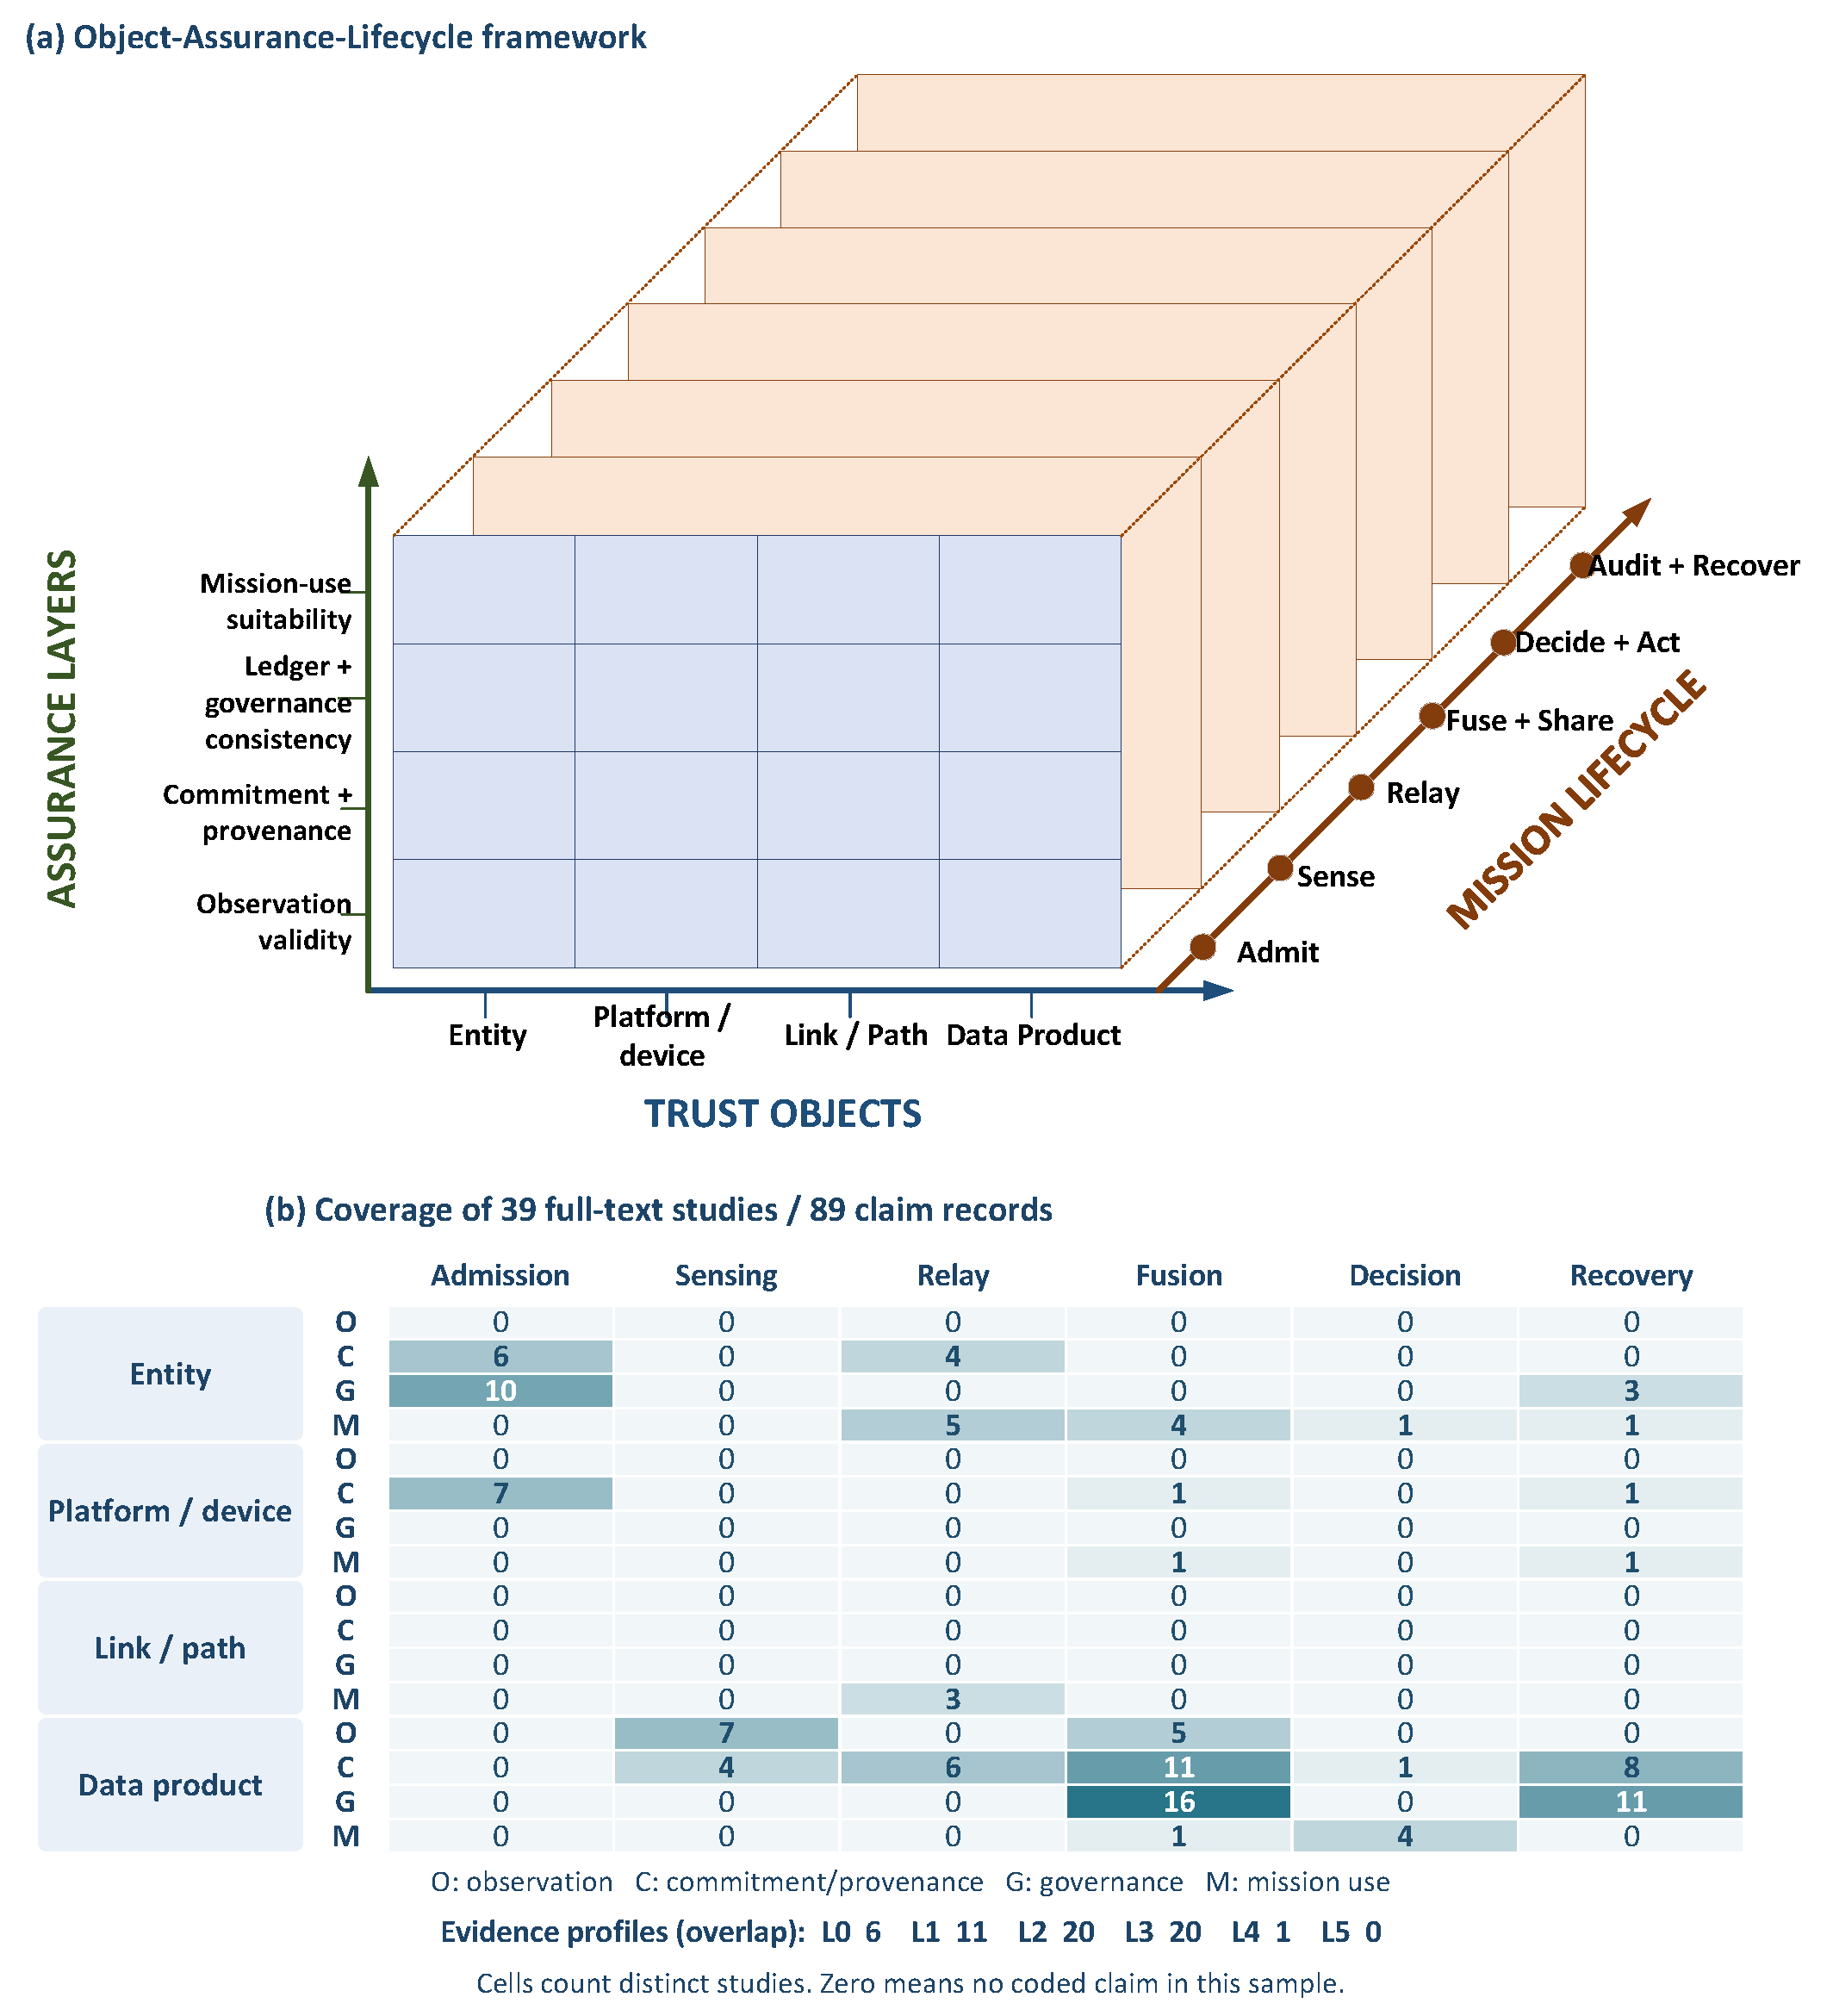
\includegraphics[width=.91\textwidth,height=.73\textheight,keepaspectratio]{figures/figure-03-oal-framework.pdf}
\caption{OAL 框架与 39 项全文机制研究的映射。（\textbf{a}）对象、保障和生命周期维度。（\textbf{b}）由 89 条限定范围的主张记录计算得到的各确切单元格中的不同研究数。证据类型计数存在重叠。零表示没有已编码主张，并不据此确定适用性或整个研究领域的空白。表~\ref{tab:sensitivity} 区分领域效应与纳入效应。}\label{fig:oal}
\end{figure}

\begin{table}[H]\small
\caption{覆盖图谱的敏感性。被覆盖单元格数是描述性计数，不是完整性评分。D/G/F 表示融合阶段的数据治理；E/G/A 表示准入阶段的实体治理。}\label{tab:sensitivity}
\begin{tabularx}{\textwidth}{@{}YrrP{32mm}@{}}\toprule
\textbf{纳入研究/编码变体} & \textbf{研究数} & \textbf{单元格数} & \textbf{最大单元格（计数）}\\\midrule
全部研究 & 39 & 25 & D/G/F（16）\\
直接领域层 & 19 & 18 & E/G/A（6）\\
可迁移层 & 20 & 20 & D/G/F（11）\\
去除四项通用共识比较研究 & 35 & 25 & D/G/F（12）\\
去除仅有概念证据的研究 & 35 & 22 & D/G/F（15）\\
直接领域层去除代理数据研究 & 18 & 17 & E/G/A（6）\\
准入身份仅归属于实体 & 39 & 25 & D/G/F（16）\\
逐一剔除研究（39 次运行） & 38 & 23--25 & D/G/F（15--16）\\\bottomrule
\end{tabularx}\end{table}

AIS 比较展示了一次保障交接。海事监测原型记录经过授权的接收机提交的观测\citep{maritime2022monitoring}；pAIS 和 SecAIS 则考察 AIS 消息保护\citep{kessler2020protected,goudossis2022secais}。pAIS 演示使用较弱的演示参数，SecAIS 则通过仿真 AIS 设备实现所选模式。它们的 L3 类型说明存在软件实现，并不意味着安全强度相同或已经完成无线实传验证。依赖这些信息的导航服务仍需获得有关所报告位置的证据。视觉里程计交叉检查提供了这样一种机制，其评估基于记录数据，并存在低纹理水面或夜间条件下的局限\citep{varshosaz2019spoofing}。多 UAV 交叉佐证在对观察者和恶意参与者作出假设的条件下，提供另一种机制\citep{garcamagario2019security,barka2022towards}。OAL 揭示了这样一个环节：如果接受规则规定不充分，带有签名、存储一致但内容错误的位置仍可能通过检查。

UAV 信任与路由研究提供了保持连续性的先例。分层无人机信任和区块链辅助路由，会随行为变化更新声誉并限制协作\citep{hierarchical2023trust,yang2023trusted}。Yang 等报告了一项限定范围的实验，涉及八个实体 UAV 节点、定时恶意转发和链路中断。这支持协作/路径调整主张（L3/L4）；其更大规模的共识基准测试使用独立容器环境。这些机制已经将行为观测与持续使用相联系。联盟场景新增的问题是：处于分区中的参与方如何解释权限变化，并将失效处理传播到依赖产品。第~\ref{sec:trace} 节进一步展开这一问题。

任务适用性同样具有特定范围。COMITMENT 将伙伴历史与工作负载/容量标准结合，用于雾计算卸载\citep{alkhafajiy2020comitment}。水下签密研究在桌面环境中评估密码运算，信任/能量路由则使用仿真\citep{zhang2026underwater,eetauv2025trust}。TAFL-UWSN 对联邦参与方和更新进行筛选，但其详细评估使用陆地 UNSW-NB15 数据\citep{tafl2026underwater}。这些结果分别支持不同的承诺或处理决策；将其迁移到声学任务，还需要信道、能耗和数据分布证据。

最后，落入同一单元格并不意味着机制可以互换。Raft 与拜占庭协议的故障假设不同\citep{raft2014,pbft1999,hotstuff2019,narwhal2022}。最初的 PBFT 原型没有实现视图变更或重传，因此其正常运行主张获得 L1/L3，而恢复主张获得 L1。这种主张层面的区分，避免把原型标签扩展到未经测试的路径。在整个样本中，没有提取出的主张证明：一个集成的空中-水面-水下任务，已经同时验证权限连续性、观测评估和依赖产品恢复。

\subsection{对选择与编码的敏感性}\label{sec:sensitivity}

表~\ref{tab:sensitivity} 汇总纳入和编码选择如何改变覆盖图谱。去除四篇通用共识论文后，25 个被覆盖单元格全部保留，领先单元格不变，其研究数降为 12。去除四项仅有概念证据的研究后，被覆盖单元格减少到 22。因此，基础设施比较研究增加了计数，而部分覆盖依赖概念性机制。去除使用陆地代理数据的研究后，直接领域层仍以准入治理为中心。

将 S01--S03 的平台身份编码行重新归为实体身份，会改变个别单元格计数，但不会改变被覆盖单元格数或领先单元格。每次逐一剔除分析都保留 D/G/F 为最大单元格，总体被覆盖单元格数为 23--25。L4 计数取决于 S31：若保守地将其限定范围的实体节点实验归为试验台，则 L4 消失，热图不变。领先单元格对移除单项研究保持稳定，而领域分层与主张层面的比较揭示了不同的组合要求。

\section{证据依赖、威胁传播与动态推理}
\subsection{带类型的对象依赖图}

令 $G_t=(V_t,E_t)$ 为一个以时间为索引的有向多重图，其节点是 OAL 对象及其版本或状态区间。关系明确其语义：实体\emph{控制}平台；平台\emph{承载}模型或\emph{产生}观测；路径\emph{传输}产品；实体对产品\emph{背书}或\emph{使用}产品；记录对另一产品\emph{作出承诺}。一次转换将其输入、输出、执行平台、责任实体、代码/模型版本和事件区间连接起来。在 PROV 中，该转换可以序列化为活动\citep{w3c2013provdm}。图~\ref{fig:dependency} 展示这些依赖及其证据状态。

\begin{figure}[!htbp]\centering
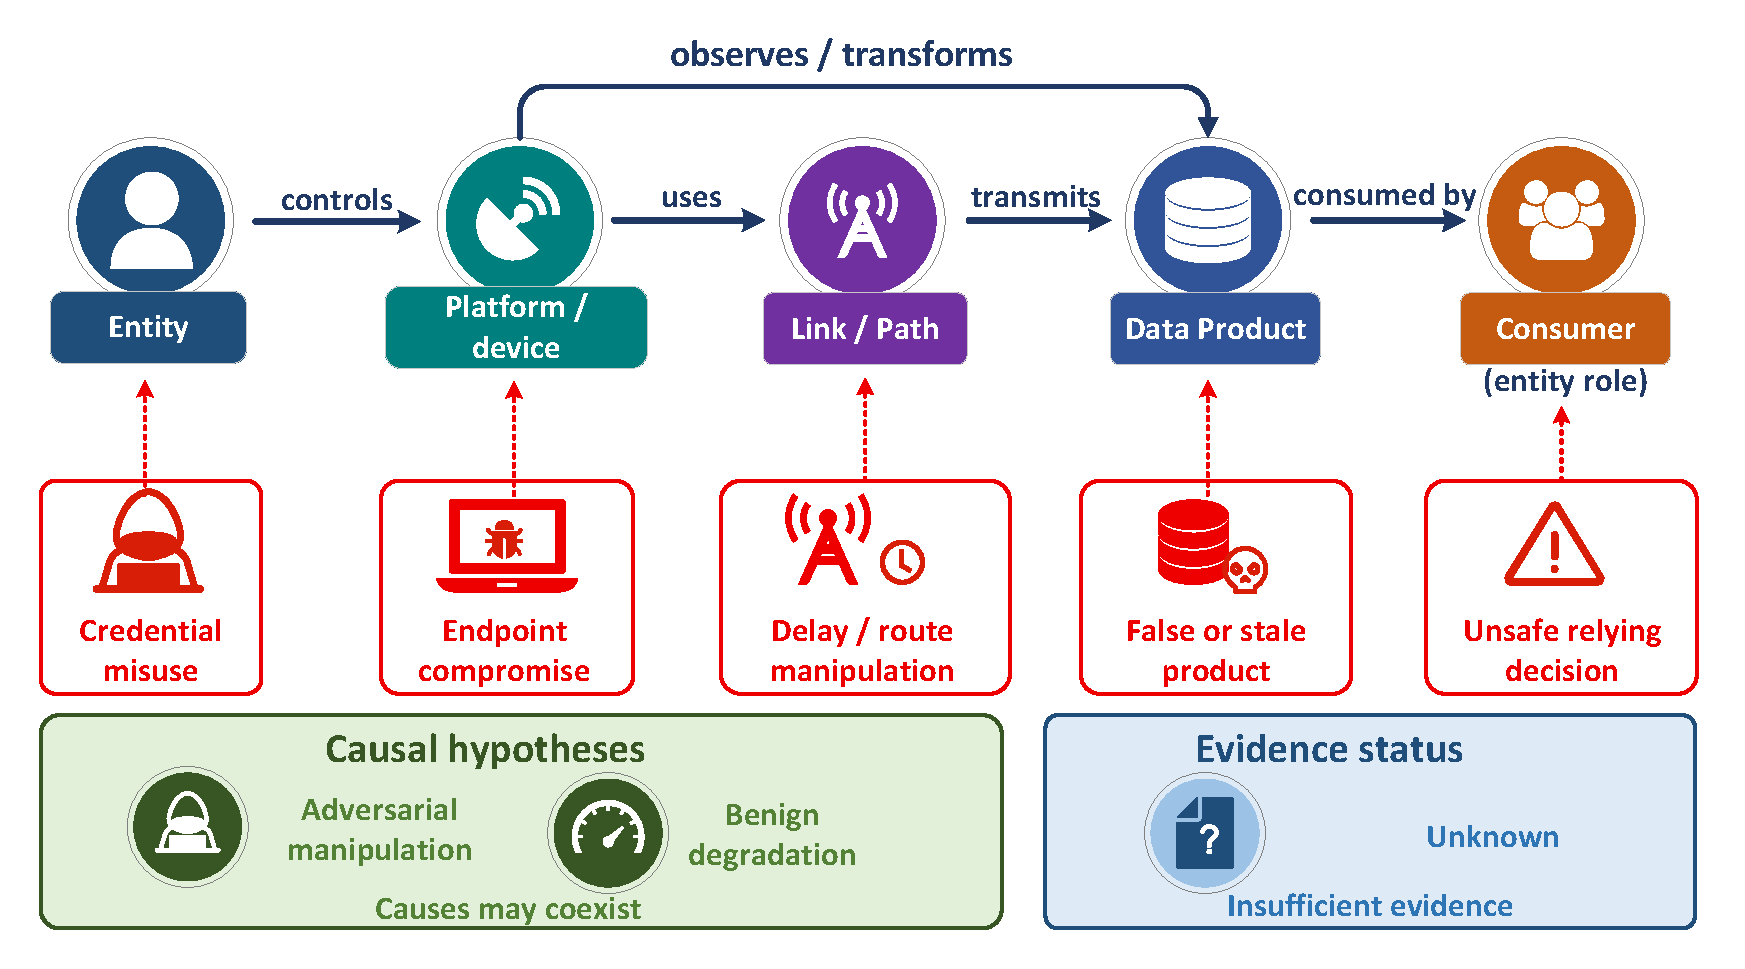
\includegraphics[width=\textwidth]{figures/figure-04-dependency-threat.pdf}
\caption{带类型的依赖与证据状态。运行关系识别假设变化所影响的主张。非恶意退化和对抗性干预属于因果假设；未知属于认识层面的结果。}\label{fig:dependency}
\end{figure}

当密钥、端点、模型或输入发生争议时，通过图遍历识别需要重新评估的主张。仅有一条图边，不能量化因果影响，也不足以支持概率更新。交叉佐证必须考虑共享的数据源、时钟、转换过程和管理根源。从同一观测派生的两个产品，并不构成两次独立观测。反之，共享中继不一定会使其他方面独立的数据源的端到端签名失效。

\subsection{威胁、退化与证据缺失}

分析陈述应识别攻击者或环境原因及其相关能力，再沿受影响对象和传播关系追踪至任务后果。同时记录控制措施和剩余不确定性。例如，被攻陷的 USV 可以扣留 UUV 批次，延迟使用者获得证据和开展审计；独立接触机会与受保护的本地计数器，可能在重连后暴露缺口。声学衰落也可能造成相同的交付症状，但原因不同。在原因归属仍未知时，可以限制对时效性敏感的用途。表~\ref{tab:threats} 汇总部分跨对象故障路径。

\begin{table}[H]\small
\caption{所选故障路径的跨对象分析。}\label{tab:threats}
\begin{tabularx}{\textwidth}{LLL}\toprule
\textbf{初始条件} & \textbf{受影响的依赖} & \textbf{证据与响应}\\\midrule
凭证被盗 & 从实体权限到签名产品 & 按生效时间撤销；审查签名的派生后代\\
端点被攻陷 & 从设备状态到观测或转换 & 证明范围、诊断与交叉佐证；隔离受影响输出\\
衰落或干扰 & 从路径可用性到证据时效性 & 信道/情境证据；限制过时信息的使用，保留原因不确定性\\
相关数据源 & 从共享输入到融合结论 & 谱系与共同原因模型；减少独立证据计数\\
治理法定人数不可用 & 从共享策略到新的全局权限 & 保留先前检查点；执行有界本地委托\\\bottomrule
\end{tabularx}\end{table}

\subsection{CTG 推理循环}

CTG 通过图~\ref{fig:ctg} 中的八步循环，利用情境、时间状态和依赖关系指导评估及策略行动。证据捕获包括绑定验证；依赖传播识别受影响的派生后代，以便在明确的推断规则下重新评估。

MAPE-K 提供监控、分析、规划、执行和共享知识\citep{kephart2003autonomic,ibm2005mapek}。CTG 将这些功能应用于主张评估，区分事件时间和接收时间，并通过已记录的依赖关系触发重新评估。JDL 融合模型区分对象、态势、影响和过程优化\citep{steinberg1999jdl}。针对这些估计，CTG 记录依赖决策所需的身份、溯源、治理和时间证据。

实现可以采用贝叶斯模型、主观逻辑、隐状态推断、规则或学习型分类器。输出保留所指属性、情境、证据谱系、不确定性和允许用途。变化后重新估计信任，需要明确的更新规则，而不是沿图边任意扣减。硬性授权条件可以与分级质量估计共存；是否将某项条件设为不可由其他指标补偿，由任务策略决定。

\begin{figure}[!htbp]\centering
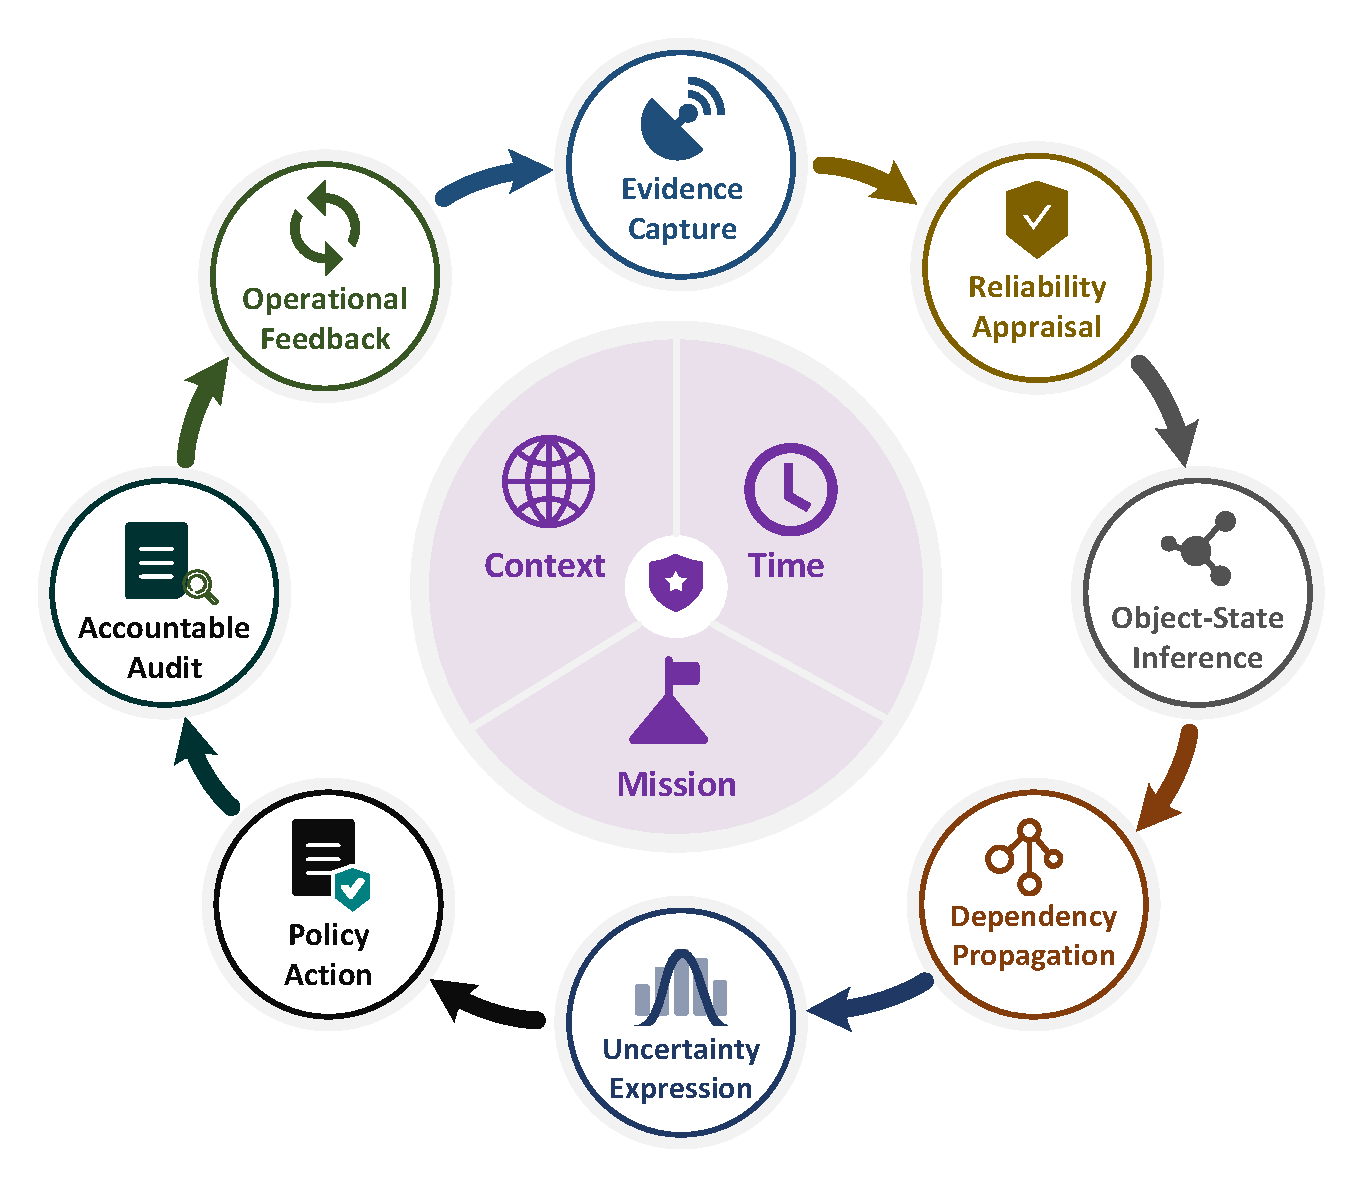
\includegraphics[width=.78\textwidth]{figures/figure-05-ctg-reasoning-loop.pdf}
\caption{CTG 评估与行动循环，各步骤共享策略、时间状态和依赖知识。}\label{fig:ctg}
\end{figure}

\subsection{分区、撤销与协调轨迹}\label{sec:trace}

第~\ref{sec:coalition} 节的联盟已共同批准策略版本 1，以及一项在 $t=480$ s 到期、适用于低后果用途的本地委托。在 $t=0$ 时，USV 失去岸端连接；在 $t=240$ s 时，岸端组织提交对一个 UUV 签名密钥的撤销，立即生效。UUV 在 $t=600$ s 重连时收到撤销信息。其受保护时钟报告事件区间，而不是精确事件时间。该场景假定保留事件具有可信的、被攻陷之前的时间/计数器记录；仅凭被盗密钥无法建立可信的历史时间戳。

三条签名记录的区间分别为 $[114,126]$、$[234,246]$ 和 $[294,306]$ s。重连后，验证方检查源签名、批次包含关系、策略纪元和撤销历史。区间在 240 s 之前结束的记录，可以具备历史审计资格；区间在 240 s 或之后开始的记录，在事件时刻已被撤销；跨越 240 s 的区间被隔离，等待复核。具备历史资格，不会授权新的物理行动，也不会使观测重新变得新鲜。

示例均值对签名有效性、观测质量、谱系、缓存策略匹配和时间权限取平均，使用 $[1,0.95,1,1,a]$，其中 $a=1,0.5,0$，阈值为 0.75。这种可补偿聚合接受全部三条记录。加入明确权限否决条件的标量策略，则产生与带类型规则完全相同的决策。决策差异源于策略是否将时间权限作为否决条件执行。表~\ref{tab:trace} 报告回放结果。

\begin{table}[H]\small
\caption{可执行回放结果。账本与具有策略验证能力的见证日志路径使用相同的证据和授权规则。标量示例使用相同的输入特征。}\label{tab:trace}
\begin{tabularx}{\textwidth}{@{}P{25mm}YP{21mm}Y@{}}\toprule
\textbf{事件区间（s）} & \textbf{OAL 组织的规则/验证日志} & \textbf{均值分数} & \textbf{标量决策}\\\midrule
114--126 & 合格的历史记录 & 0.99 & 均值接受；带否决条件的标量与规则一致\\
234--246 & 隔离：与撤销时点重叠 & 0.89 & 均值接受；带否决条件的标量将其隔离\\
294--306 & 在事件时刻已撤销 & 0.79 & 均值接受；带否决条件的标量拒绝\\\bottomrule
\end{tabularx}\end{table}

断连期间，420 s 时的行动可在缓存运行边界内获得受限本地权限，即使后续审计发现其与已生效的全局撤销相冲突；到 540 s 时，该边界已到期，本地策略拒绝行动。协调过程同时保留当时本地可用的权限与后续全局判断。若改写旧决策，仿佛航行器在 240 s 时就收到了撤销信息，就会抹去这一区别。

合成回放验证 Ed25519 签名与 Merkle 包含关系，拒绝遭修改的记录/证明，检查带重复交付的全部六种到达顺序，并枚举联盟签名者的全部 16 个子集。账本策略与验证日志的决策函数在所有情况下均一致。第~\ref{sec:pattern} 节说明相同的应用规则如何映射到 Fabric，以及资源受限航行器如何接收可审计结果。

\section{区块链辅助保障：选择与明确的实现模式}
\subsection{使用账本的决策}\label{sec:ledger-choice}

账本采用决策从写入者、状态和权限出发。W\"ust 和 Gervais 围绕是否需要存储共享状态、写入者数量及其信任关系，以及可信参与方的可用性组织决策\citep{wust2018need}。Locher 等考察可信第三方的哪些功能可以由分布式一致性替代\citep{locher2018when}。对于任务保障，相关要求是：任何单一组织都不能悄然改变已接受的成员资格、策略或撤销历史，同时授权参与方保留可相互验证的状态。

在联盟示例中，A 不能独自替换传感器接受策略，C 不能在网关事件发生后删除此前已确认的批次，D 也不能自行宣布其数据已获联盟接受。四个独立组织可以共同验证这些转换。许可账本是实现这一要求的一种方式。

最强的替代方案是一种透明服务，其检查点和状态转换由独立见证方按照相同授权规则检查。该服务可以满足相同的安全性要求。仅检查一致性的见证方能够发现或暴露不一致历史，但这一行为本身并不能证明策略变更已经获得授权。增加共同策略验证可以补足这一环节。因此，第~\ref{sec:trace} 节的回放发现，账本与策略验证日志产生等价决策。架构选择随后取决于实现复杂度、隐私、可用性、恢复和实测成本。图~\ref{fig:blockchain-boundary} 汇总这种共享状态服务选择。

治理可行性同样是采用条件。TradeLens 虽然在技术上可行，但未能实现所需的全球行业协作和商业可行性，Maersk 与 IBM 因而终止了该平台\citep{maersk2022tradelens}。这一海事案例说明需要评估激励、参与、退出和运行责任。

\begin{figure}[!htbp]\centering
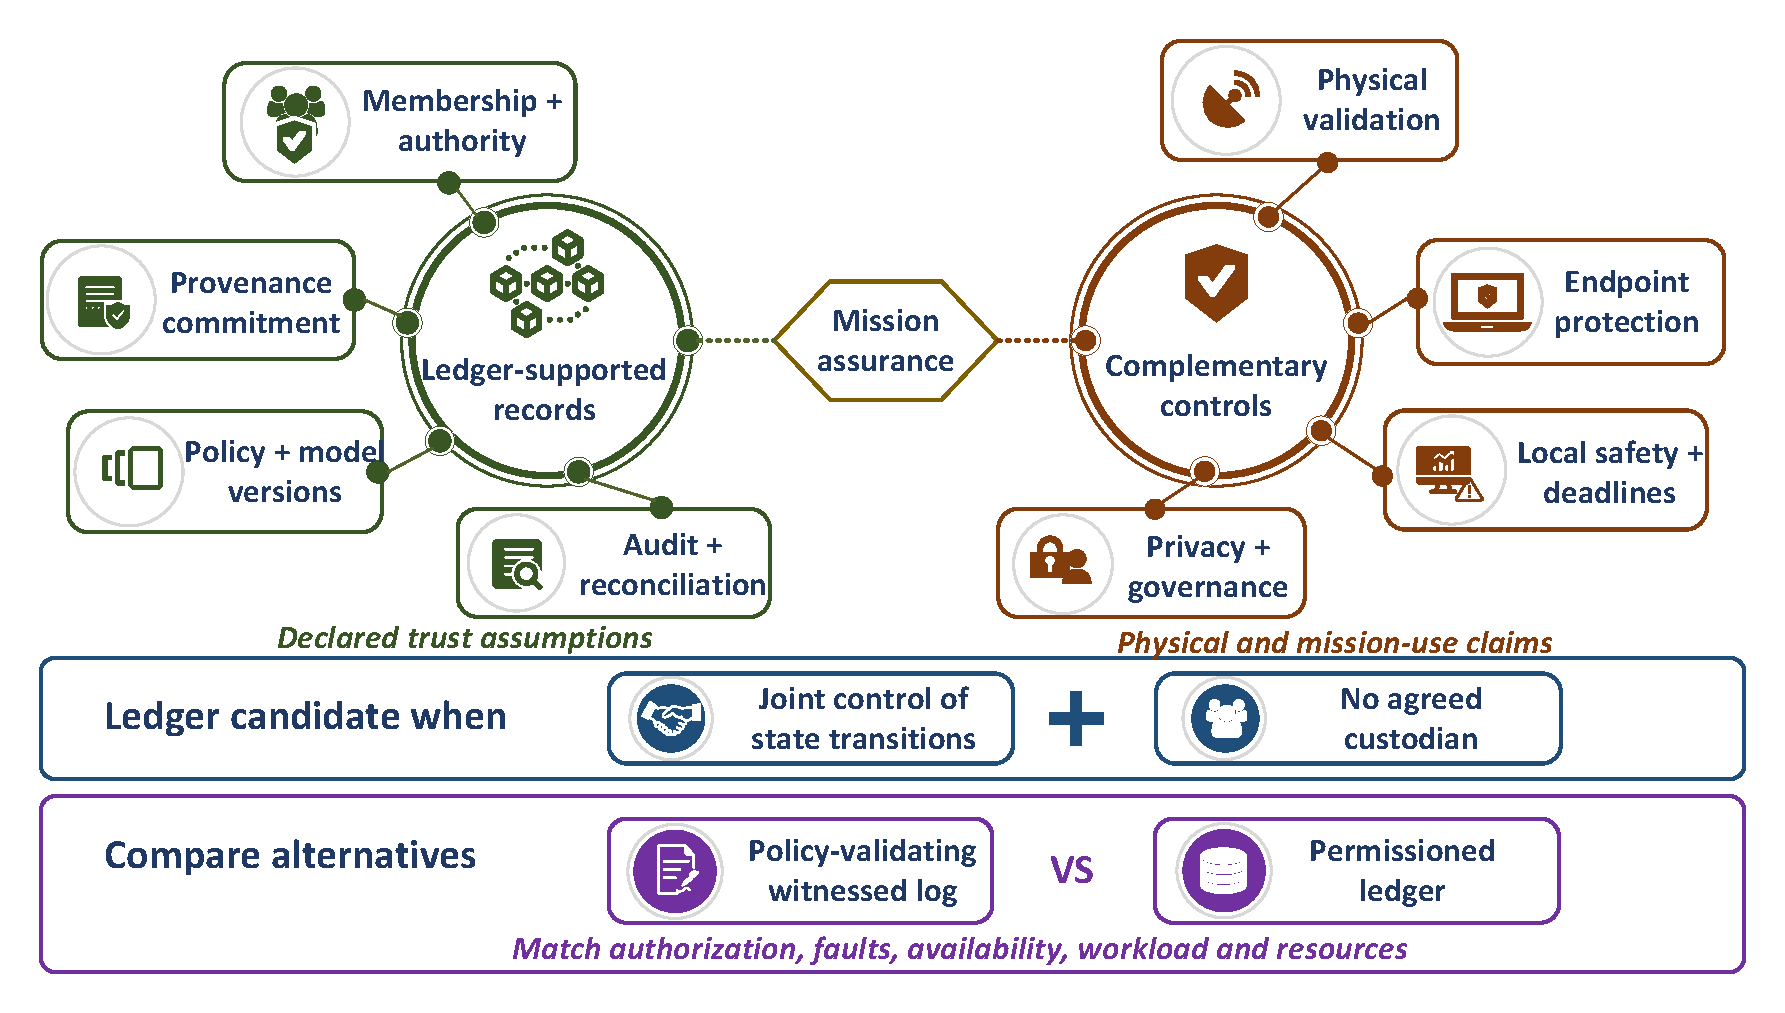
\includegraphics[width=\textwidth]{figures/figure-06-blockchain-boundary.pdf}
\caption{基于需求的共享状态服务选择。在匹配的治理保障条件下，比较具有策略验证能力的见证日志与许可账本。物理评估与本地安全仍由应用负责。}\label{fig:blockchain-boundary}
\end{figure}

\subsection{任务要求与候选共识机制}\label{sec:consensus}

如 \v{S}varcmajer 等所倡导\citep{svarcmajer2026consensus}，基于需求的选择流程在选择协议前先明确故障模型。此处联盟设计假定：四个独立控制的岸端节点中，至多存在一个拜占庭管理域。在 USV 分区期间必须保持安全性；当无法获得有响应的法定人数时，新的全局决策可以停止。示例协调截止时间为事件可供岸端处理后的 60 s。一次任务期间成员保持稳定，并通过共同批准的纪元转换来变更。岸端节点具有足够的计算和供电能力；UUV 不参与共识。共识流量使用岸端/无线电基础设施，只有紧凑的证据承诺经过声学链路。

表~\ref{tab:consensus} 比较代表性协议类别。正常路径消息复杂度是一项选择指标，其含义取决于批处理、签名聚合、传播和视图变更。容错能力与活性假设仍具有决定作用。尤其是，采用有向无环图（DAG）组织数据，并不能免除明确说明由何种一致性协议对数据排序或认证的要求。

Raft 和拜占庭协议解决不同的故障问题\citep{raft2014,pbft1999,hotstuff2019}。CometBFT 使用自身基于轮次的共识和 gossip 传播规则\citep{cometbft2026}；Narwhal 是传播/内存池组件，Tusk 则提供关联的排序协议\citep{narwhal2022}。BUS 所实现的基于权威节点的 UAV 采集，展示了将功能部署在能力充足的验证节点上的做法\citep{islam2019bus}。轻量级 IoT 方案同样支持将共识移出受限端点\citep{dorri2017towards}；评估这种优化时，需要同时考虑由此形成的管理依赖。

\begin{table}[H]\footnotesize
\caption{候选共识机制与任务要求的比较。消息复杂度阶数描述代表性的正常路径；恢复成本可能更高。}\label{tab:consensus}
\begin{tabularx}{\textwidth}{@{}P{25mm}YYY@{}}\toprule
\textbf{类别} & \textbf{故障模型与分区行为} & \textbf{时延、流量及资源影响} & \textbf{适用场景}\\\midrule
Raft & 崩溃故障；推进需要多数节点 & 领导者复制，每条记录通常为 $O(n)$ 次交换；服务器成本低；受管理的成员变更 & 单一责任运营方及仅考虑崩溃的副本；不足以应对拜占庭联盟管理方\\
经典 BFT / SmartBFT & 拜占庭故障；通常要求 $n\geq3f+1$ 和 $2f+1$ 个有响应的投票 & 多阶段通信，通常为 $O(n^2)$；超时/视图变更成本；能力充分且稳定的节点 & 小型独立岸端联盟；本文选择的 Fabric 排序候选\\
HotStuff & 拜占庭故障；法定人数及部分同步条件下的活性 & 法定人数证书和流水线带来线性正常路径通信；密码聚合与领导者可用性重要 & 经实测证明负载收益的较大型高能力联盟\\
CometBFT & 拜占庭故障；超过三分之二投票权；轮次/锁定规则 & Tendermint 风格的提议/投票与 gossip；延迟下会发生超时；传播成本取决于实现 & 应用特定的复制状态机；不能仅因同属 BFT 就归为 HotStuff\\
基于权威节点 & 具名验证者；韧性取决于具体协议 & 挖矿成本低；必须明确调度/最终性及法定人数假设 & 只有具体权威协议满足故障要求时，才适用于受控联盟\\
基于 DAG（Narwhal/Tusk） & 可靠数据传播加明确的 BFT 排序协议 & 并行传播与存储；仍需考虑异步推进假设与通信成本 & 有资源证据支持的高吞吐岸端服务；不能绕过声学分区问题\\
面向 IoT 的设计 & 常采用簇头、可信管理者或受限验证者集合 & 将端点工作转移到高能力节点；信任与可用性假设随之变化 & 网关介导的数据采集；仅当其委托信任符合任务需求时选择\\\bottomrule
\end{tabularx}\end{table}

基础设施与应用的故障假设分别陈述。拜占庭排序服务关注副本任意行为下的一致性，并不能阻止获授权生产者提供虚假观测。背书限制谁可以批准拟议状态更新，链码则定义被批准的确定性规则。合约可能一致地执行一条不适当的规则，因此策略批准还需要有关任务后果的证据。应用必须明确紧急权限能否绕过通常的背书，以及如何记录和审查该例外。没有明确例外时，必需签名方不可用就意味着有意停止授予新的全局权限。

分区容忍性也有两层必须区分的含义。安全性是在消息延迟或不可用时，保留一致的已接受历史。可用性关注特定请求能否在截止时间前取得所需排序和应用批准。USV 断连时，岸端法定人数仍可能正常工作，从而允许岸端撤销继续推进，而 UUV 依据缓存权限运行。若岸端法定人数本身被分割，即使网关恢复连接，新的全局更新仍可能停止。评估应独立改变这两种分区位置。经典的一致性/可用性结果为网络分区下的这一区分提供动机\citep{gilbert2002brewer}；它们并不规定航行器的本地安全策略。

由此得到三种场景决策。单机构检查任务可以采用经过认证的数据库或见证日志，并增加 Raft 复制以获得崩溃故障下的可用性。四组织响应任务需要拜占庭排序加共同应用授权，或者等价的验证日志；当前 Fabric SmartBFT 是一个具体候选\citep{fabric2026bft}。断连的 UUV 群体使用签名本地记录、存储转发传输和有界委托，不要求声学共识。增加验证者数量，只有在增加独立故障域且保持法定人数可达时才有帮助。实际时延和能耗必须针对所选部署测量。

\subsection{联盟溯源与撤销模式}\label{sec:pattern}

该明确模式将证据承诺与分区后协调相结合；表~\ref{tab:blockchain-patterns} 将其与成员资格、版本协调和审计联系起来。

\begin{table}[H]\small
\caption{账本角色及其对应的应用要求。}\label{tab:blockchain-patterns}
\begin{tabularx}{\textwidth}{@{}P{24mm}YY@{}}\toprule
\textbf{角色} & \textbf{共享状态} & \textbf{所需互补证据}\\\midrule
成员资格 & 角色、委托、密钥纪元 & 身份证明与受保护的密钥保管\\
承诺 & 批次根、序列号、保留对象引用 & 签名源记录和可检索的载荷\\
版本协调 & 策略/模型哈希和批准纪元 & 模型验证与部署证据\\
审计 & 决策、证据链接和生效时间历史 & 完整捕获与独立审查\\
协调 & 已收到批次、缺口、冲突和判断 & 受保护的时钟/计数器与离线权限历史\\\bottomrule
\end{tabularx}\end{table}

\textbf{部署与背书。}A--D 各组织在能力充分的岸端基础设施上，分别部署一个背书对等节点和一个独立排序节点。示例 BFT 服务包含四个排序节点，在其协议假设下容忍一个拜占庭节点。管理上的分离提供独立故障域。应用背书规则为 \texttt{AND(A, B, OR(C, D))}；通道配置和链码定义批准要求相同的联盟权限。A 和 B 是必需方，因此即使仍有三个排序节点响应，应用也可能停止推进。USV 负责转发和缓存签名证据，没有共识投票权。分区中的网关缓存批次，并在重连后进行幂等重试。UUV 安全控制始终遵循其本地运行边界。

\textbf{状态与编码。}状态键包括 mission/policy/epoch、producer/key/history、delegation/identifier、batch/producer/sequence 和 judgment/record/policy，分别表示任务/策略/纪元、生产者/密钥/历史、委托/标识符、批次/生产者/序列，以及判断/记录/策略。定长源记录体包含：各一字节的版本与类型、两个 16 字节的任务/生产者标识符、各四字节的序列与权限纪元字段、两个八字节的事件时间边界，以及三个分别对应策略、载荷、父项/根的 32 字节哈希。这些字段合计 154 字节。整数采用网络字节序；时间为相对于声明的任务纪元的有符号秒数。加上 64 字节 Ed25519 签名后，一条记录为 218 字节。域分离签名和哈希绑定记录类型与版本。批次采用相同的记录体布局，使用 Merkle 根和前一批次根，并增加两字节的记录数：签名前为 156 字节，签名后为 220 字节。十条签名记录保留在链下。网关的规范化 JSON 应用载荷为 525 字节。

\textbf{确定性的链码操作。}\texttt{CommitBatch} 读取任务纪元、网关角色和最新批次序列；验证紧凑网关签名与策略绑定；拒绝不一致序列或标识符相同而内容不同的重复项；并记录根。内容完全相同的重试返回已有结果。这提交的是可审计批次，并不声称每个叶记录都适合使用。\texttt{JudgeRecord} 验证提交的源签名和包含证明，读取生产者的历史密钥状态与委托，并依据第~\ref{sec:trace} 节的区间规则，写入独立的合格/已撤销/已隔离判断。\texttt{UpdatePolicy} 和 \texttt{RevokeKey} 要求联盟背书规则和单调递增纪元；撤销记录保留生效时间。决策读取的所有状态均进入 Fabric 读集，使验证能够拒绝基于过时状态的并发更新。链码执行期间不获取外部时钟或预言机值；这些输入由获授权提交的证据提供。

\textbf{提交状态与受限验证。}Fabric 的排序先于对等节点验证，因此区块包含关系并不能证明世界状态更新有效\citep{androulaki2018hyperledger,hyperledger2026fabric}。观察到有效提交后，满足 A+B+（C 或 D）的三个不同组织签署应用回执，内容包括任务、策略/权限纪元、批次根、序列、事件跨度和记录数。回执签署代码必须检查提交验证状态及预期应用状态。UUV 根据固定信任的纪元检查授权签名者身份、签名、单调递增的检查点序列、源记录签名和 Merkle 分支。十个叶节点补齐至 16 个时，分支包含四个 32 字节哈希。这些检查在固定信任的密钥下，建立共同证明的应用检查点与包含关系；它们不构成对全部 Fabric 共识和对等节点验证执行过程的原生验证。新纪元需要来自当前固定信任纪元的经过认证的转换。回执构成额外的应用信任边界，需要实现和测试。

\subsection{通信预算与分区敏感性}\label{sec:budget}

回执路径与检索路径满足不同的证据需求。收到检查点的航行器可以验证：独立组织在固定信任的权限纪元下确认了已提交的根。要评估观测，它仍需获取相关叶记录、包含路径，以及必要的数据源或转换证据。因此，只传递承诺的接触时段所支持的主张，比完整证据交付更窄。检索策略可以优先处理近期且后果重大的产品，把大批量图像推迟至更高带宽的接触时段，同时记录哪些必需输入仍不可用。检索失败表示证据缺失，不能表示完整性检查成功。

时钟与密钥转换也影响证明的可用期限。新策略发布后，缓存检查点仍是历史承诺的证据，但它能否支持新决策，取决于依赖策略和经过认证的转换历史。时钟不确定的航行器不能仅检查账本根，就认定到期条件仍然成立。它需要有界时间区间，或采用更严格的后备策略。同样，新的回执也无法使不可信的采集时间戳变得可信。这些要求将应用层证明与回放所使用的相同时间假设绑定，并明确受限验证方在这些假设失效时必须采取的行动。

Ed25519 签名长度为 64 字节\citep{rfc8032}；ML-DSA-44 签名长度为 2420 字节\citep{fips204}。预算比较这两种紧凑应用签名配置。Fabric 注册证书、背书、提案响应、读写集和信封，会增加取决于部署的字节量。只有网关在岸端网络上传输这些完整事务。完整事务大小和资源成本取决于配置的 Fabric 实现；525 字节的 JSON 数值仅覆盖网关的应用载荷。

对于大小为 $B$ 字节、净载荷速率为 $R$ bit/s 的消息，串行化传输时间下界为 $8B/R$。表~\ref{tab:budget} 使用 100、1000 和 5000 bit/s 作为场景输入。计算不包含传播、等待接触、调制解调器成帧、BPSec 开销、丢失、重试，以及证书/纪元更新。这些因素会增加端到端时延，必须针对明确的调制解调器与传输配置另行加入。

\begin{table}[H]\small
\caption{应用消息串行化传输时间下界。所有大小均由第~\ref{sec:pattern} 节的编码计算；ML-DSA 数值通过替换为标准化签名长度得到。}\label{tab:budget}
\begin{tabularx}{\textwidth}{@{}Yrrrr@{}}\toprule
\textbf{消息} & \textbf{字节} & \textbf{100 bit/s} & \textbf{1 kbit/s} & \textbf{5 kbit/s}\\\midrule
Ed25519 源记录 & 218 & 17.44 s & 1.744 s & 0.349 s\\
Ed25519 批次承诺（10 条记录） & 220 & 17.60 s & 1.760 s & 0.352 s\\
十条完整 Ed25519 记录 & 2180 & 174.40 s & 17.440 s & 3.488 s\\
ML-DSA-44 批次承诺 & 2576 & 206.08 s & 20.608 s & 4.122 s\\
Ed25519 记录+分支+共同回执 & 697 & 55.76 s & 5.576 s & 1.115 s\\\bottomrule
\end{tabularx}\end{table}

697 字节的下行内容包括：218 字节源记录、128 字节分支、两字节叶索引、156 字节检查点、一字节签名者位图，以及三个 64 字节签名。按每分钟一个十记录批次计算，220 字节承诺平均需要约 29.3 净 bit/s，而发送全部十条签名记录需要约 290.7 bit/s。因此，只传递承诺可以适应某些无法承载完整证据的接触时段，代价是需要后续检索，且即时评估不完整。以相同频率发送一个含十条记录的 ML-DSA-44 批次承诺，需要约 343.5 bit/s。假定公钥已预先配置；密钥分发与后量子验证时间属于另行计算的成本。

分区敏感性计算覆盖 63 种配置：验证者数为 4、7 和 10；响应数分别为法定人数减一、法定人数，以及全部验证者；分区持续时间为 0、10、30、58、59、60 和 120 s。假设恢复接触后的延迟分别为账本路径 2 s、验证日志路径 1 s，在法定人数可达时，60 s 截止时间分别容许最长 58 s 和 59 s 的分区。低于法定人数时，两者都不能完成新的共同决策。除排序法定人数外，还必须检查应用背书可用性。

\section{评估实践与证据成熟度}
\subsection{针对具体主张的证据类型}

L0--L5 记录主张如何得到支持：概念、分析、仿真/数据、原型、现场试验和持续运行。图~\ref{fig:maturity} 将每种证据形式与其输入、推理或评估，以及输出相联系。形式上的正确性、实验控制、环境代表性和运行持续时间，仍是相互独立的评估维度。

\begin{figure}[!htbp]\centering
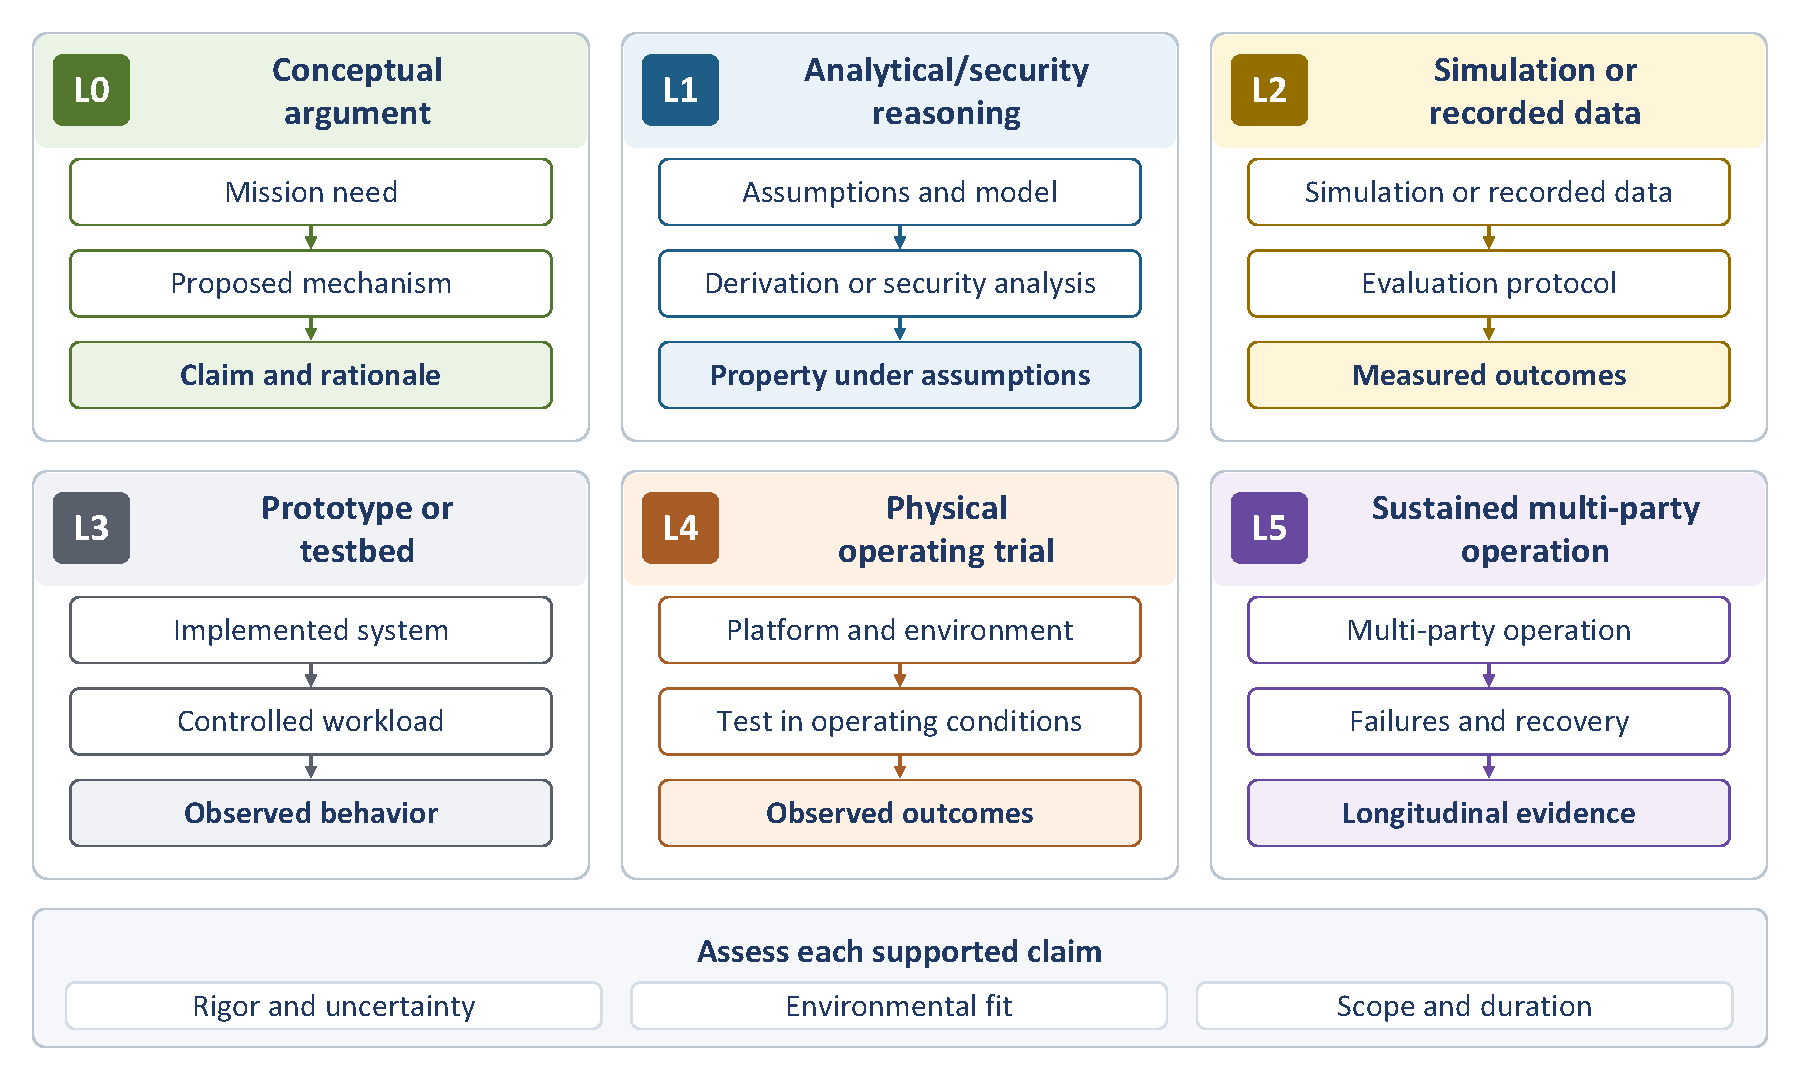
\includegraphics[width=\textwidth]{figures/figure-07-evidence-maturity.pdf}
\caption{互补的证据形式及其对具体主张的支持。各面板连接输入、推理或评估，以及输出；严谨性、环境适合性和范围分别评估。}\label{fig:maturity}
\end{figure}

在 39 项研究样本中，6 项的证据类型包含 L0，11 项包含 L1，20 项包含 L2，20 项包含 L3，1 项包含 L4；没有研究包含 L5。类型存在重叠；4 项研究仅有概念证据。L4 归类针对 S31 限定范围的实体 UAV 节点协作/路由实验；其容器共识基准测试仍为 L3。第~\ref{sec:sensitivity} 节将仅把该实验归为 L3 作为敏感性变体进行评估。BUS 提供硬件原型证据，而记录的 GNSS 轨迹支持 L2。这些环境回答有关实现、实体运行和迁移的不同问题。

如第~\ref{sec:comparative} 节的比较所示，证据形式、参数强度、实际测试的机制和环境相关性，共同决定所支持的主张。

\subsection{数据集、仿真器与试验台}

公共资源支持互补的评估任务。CICIoT2023、TON\_IoT 和 Edge-IIoTset 提供攻击与遥测数据，用于分类和鲁棒性测试\citep{neto2023ciciot2023,alsaedi2020ton,ferrag2022edge}。SeaDronesSee 提供海事视觉数据\citep{varga2022seadronessee}。AirSim、UUV Simulator 和 Aqua-Sim NG 分别面向载具/传感器仿真、水下动力学和水下通信\citep{shah2018airsim,manhaes2016uuv,martin2017aqua}。在同一实验中使用它们，需要兼容的时钟、几何、运动性和事件接口，并配套经过独立验证的任务损失模型。表~\ref{tab:evaluation} 汇总这些资源和迁移检查。

\begin{table}[H]\small
\caption{评估资源与所需的迁移检查。}\label{tab:evaluation}
\begin{tabularx}{\textwidth}{LLL}\toprule
\textbf{资源} & \textbf{有用证据} & \textbf{所需补充}\\\midrule
IoT 攻击/遥测数据集 & 检测、校准、缺失情况和错误隔离 & 海事拓扑、非恶意退化和任务后果\\
SeaDronesSee / GNSS 记录 & 视觉检测或信号评估 & 针对所述物理主张的独立真实值\\
AirSim / UUV Simulator & 动力学、传感器、扰动与控制 & 所配置模型的现场有效性\\
Aqua-Sim NG & 路径时延、丢失、能耗和接触行为 & 物理观测与治理模块\\
账本与见证日志试验台 & 验证、字节量、时延、恢复和成员变更 & 匹配的保障、证据工作负载和故障域\\
多组织现场演练 & 集成决策、恢复和审计 & 重复场景与明确的运行持续时间\\\bottomrule
\end{tabularx}\end{table}

\subsection{指标、基线与可复现性}

评估应测量推断误差与不确定性、任务后果、网络/资源成本、共享状态行为和问责能力。任务结果包括不安全接受、错误隔离关键中继、任务完成、安全约束违反，以及截止时间未满足。资源指标包括每个证据事件的字节量、能耗，以及背书/提交时延。问责指标包括识别受影响派生后代所需的时间，以及具有可检索溯源的决策比例。仅报告吞吐量，会遗漏及时但不适当的决策所造成的后果。

场景因素包括实体与设备分别被攻陷、独立与相关观测、衰落与干扰、新鲜与过时的证明、接触丢失、合谋，以及不同的权限到期期限。真实状态区分非恶意退化、对抗性干预及两者共存；未知是评估结果。训练、调参、校准和评估使用相互分离的数据，并在划分时考虑共享任务、平台和记录时段。配对场景以及基于独立运行的不确定性区间支持比较性主张。未交付事件和未满足截止时间的事件，仍纳入时延/可用性分析。

基线接收相同的原始证据、行动集合、任务目标和调参预算。评估方法比较包括带明确授权否决条件的标量模型，以及针对谱系、共同原因和不确定性的组件消融。存储/治理比较包括经过认证的数据库、独立见证的一致性日志，以及具备策略验证能力的共同签署日志。最强基线在管理独立性、法定人数、留存和生效时间语义上保持匹配。在解释成本差异之前，先报告保障差异。

复现需要拓扑、故障域以及信道/接触模型。实现说明应给出软件与策略/模型版本、载荷编码、密码套件和背书规则。工作负载、随机种子、真实值和任务损失权重共同定义评估条件。

评估还应区分采集完整性与记录一致性。测试可以维护独立的事件真值源，然后注入签名前遗漏、删除尚未被见证的后缀、承诺后的中继扣留，以及根已被接受后的链下对象丢失。这些故障的可观测性不同。保留的回执可以暴露已确认批次的缺失；却无法揭示从未被任何可信观察者捕获的事件。因此，指标应分别报告预期被捕获的事件基数、得到见证方确认的事件、按共同策略提交的事件，以及载荷仍可检索的事件。这区分了保存、检测和恢复，而不将三者合并成单一审计成功率。

恢复工作负载需要同样的精确性。返回的网关可能携带有效的旧观测、使用已撤销密钥的提交、冲突序列号，以及在不同策略版本下生成的记录。只对无异常插入进行基准测试，会遗漏这种混合情况。实验应改变积压数据的年龄与规模、被攻陷密钥的截止时点、重复率、纪元转换、证明检索，以及需要人工复核的比例。同时报告自动处理时间，以及应用能够依据已解决判断采取行动之前的时间。共享状态吞吐量可以保持很高，但语义协调仍可能被证据缺失或必需背书方不可用所阻塞。

最后，推断策略比较应保留行动成本。隔离所有不确定观测可以减少不安全接受，却可能阻止有用任务执行。明确的损失模型应为不安全依赖、不必要隔离、任务推迟、佐证请求和人工复核赋予成本。结果应展示对这些权重，以及攻击和非恶意退化发生率的敏感性。校准和决策损失回答不同问题：校准良好的估计仍可能被不适当的策略使用，而保守规则可以在不输出概率的情况下作出安全决策。分别评估二者，遵循了式~\eqref{eq:trust} 中的评估/决策接口。

\section{讨论与研究议程}
\subsection{集成、治理与隐私}

机制组合同时需要针对具体主张的策略与依赖分析。架构中的共同原因仍会产生影响：增加 UUV 数量，并不能消除它们对同一网关、时钟或运营方的依赖。

联盟设计必须规定准入、合约/模型批准、紧急权限、争议、成员退出和审计责任。海事采用研究与 TradeLens 经验说明，参与和激励为何需要纳入这项分析\citep{zhou2020key,farah2024survey,maersk2022tradelens}。示例中的背书规则保留共同控制，同时通过必需签名方产生可测量的可用性成本。同一所有者控制的更多副本，不会形成更多独立治理域。

跨行业研究区分可追溯性收益与实现这些收益所需的组织变革\citep{kshetri20181,lnes2017blockchain}。联盟协议分配留存、披露、维护和事件响应职责，包括成员退出后的证据可用性，以及密钥轮换后的历史签名处理。比较账本与验证日志时，必须匹配这些治理规定。

隐私取决于载荷加密之外的因素。稳定标识符、路径托管、背书时序和模型使用记录，可能泄露无人平台活动与组织关系\citep{reyna2018blockchain,kshetri2017can}。因此，可审计性需要同时配备数据最小化、选择性披露、留存规则和受控身份解析。撤销依据策略使未来依赖失效；它不会删除已保留的承诺。人工覆盖决定是一项另行授权并记录的转换，应包含证据、理由和后果。

\subsection{可证伪的研究命题}\label{sec:propositions}

以下命题定义未来的比较测试。每个实验预先规定任务分布、最小有用效应、主要结果和分析规则。零效应和不利结果能够识别附加结构不产生收益的条件。

\textbf{P1（主张组织）。}检验保障向量能否在匹配的错误隔离与时延预算下，相对于调优后的标量策略，降低留出测试中的不安全接受。两者接收完整证据、相同行动集合和相等调参预算；标量包含授权/时效性门控与交互项。若比较方法表现相同或更好，则命题被否证，表~\ref{tab:trace} 中带否决条件的标量就是这样的例子。

\textbf{P2（依赖建模）。}在预先规定的共享源误差和合谋率下，检验含共同原因变量的模型，相对于同等调优的独立性模型，是否改善适当评分规则和任务损失。纳入正确、不完整和错误谱系条件。当模型设定错误或采集成本抵消收益，或观测足够独立以至于不存在有用改进时，命题不成立。

\textbf{P3（诊断与未知状态）。}在退化、攻击和证据中断混合发生时，比较保留非恶意、对抗性和未决假设的模型与二元评估模型。两者都可以选择相同行动，包括弃权。分别消融诊断与弃权功能，并测量不安全接受、错误隔离、佐证延迟和可用性损失带来的损失。若增加诊断状态导致损失上升，或未带来有用改进，则命题不成立。

\textbf{P4（离线权限）。}改变委托范围、到期时间、时钟不确定性、分区持续时间和撤销时点。与仅允许新获取全局授权，以及不受限制的离线自主运行相比，检验有界委托是否能够在截止时间前完成的任务与违反已生效全局策略的行动之间，提供有用的权衡。分别报告本地获授权行动与事后发现冲突的行动。若某些运行条件下，有界策略在这两个结果上都被其他方法支配，则包括在命题失败的情形中。

\textbf{P5（条件性的账本价值）。}在匹配成员资格、故障、规则、留存和工作负载的条件下，比较已实现的账本与独立见证日志服务。改变 $n$、有响应的法定人数、分区持续时间 $D$、事件率和积压量。对于截止时间 $\tau$，使用在负载 $\lambda$ 下实测的恢复接触后延迟 $L$，估计 $D+L(n,\lambda)\leq\tau$。在固定字节/能耗预算下，检验及时可验证决策或恢复完整性的改进。若安全性相同但成本更高、背书方可用性更低，或相对于日志没有改进，则该运行条件下的优势被否证。第~\ref{sec:budget} 节的 58/59 s 边界使用的是假定延迟。

\textbf{P6（评估覆盖）。}在相同候选集合与相等评估预算下，分别仅使用事务/网络指标，或在其基础上加入观测、端点、治理和任务结果，来选择配置。按固定选择规则比较留出测试中的任务损失。若计入额外采集与解释成本后，更全面的评估未改善选择，则命题不成立。

\subsection{保障论证与海事要求}\label{sec:assurance-case}

OAL 提供保障论证的内容，已有表示法提供其结构。GSN 表示主张、策略、情境、假设和证据，SACM 则提供结构化保障论证元模型\citep{gsn2021,sacm2023}。UL 4600 提供自主产品的安全论证要求，而非图形表示法\citep{ul4600}。OAL 可以用对象/版本、保障层、生命周期阶段、事件区间和证据类型标注它们的主张。符合性评估仍与适用标准的要求相关联。

航线重规划的适用性需要可信观测、受保护的派生过程、有效权限、当前策略和可接受的不确定性。论证记录观测、签发、接收和到期时间，包括缓存权限。输入更正或密钥撤销会触发派生后代审查，同时保留具有独立支撑的产品。验证应测量证据缺口、对植入的无效论证的检测、审查者错误，以及识别受影响产品所需时间。

海事要求增加了特定应用边界。IMO 的海上自主水面船舶（MASS）试验临时指南和监管范围界定工作，提供试验与监管背景\citep{imo2019trials,imo2021scoping}。非强制性 MASS 规则于 2026 年 5 月通过，并于 2026 年 7 月 1 日生效\citep{imo2026mass}。DNV-CG-0264 面向自主及遥控船舶\citep{dnv2024autonomous}。保障论证必须明确这些文件所适用的船舶和作业、责任主管机构、运行设计条件、人员/远程控制职责，以及安全回退证据。其海事适用范围不能整体移用于 UAV 或水下作业。账本记录可以追踪批准或运行限制；实质性安全证据和适用审批流程仍需分别处理。

\subsection{迈向跨域无人系统信任配置规范}

提出的\CDUTP{}是一项关于版本化主张与证据引用的互操作研究议程。它可以复用 RATS 角色、W3C PROV 关系、零信任策略概念和安全更新清单\citep{birkholz2023remote,w3c2013provo,rose2020zero,ietf2020suit}。UAS 与海事服务规范提供通信背景\citep{threegpp22125,threegpp22119}。一个配置规范实例记录对象/类型、限定范围的主张、签发方和依赖角色、证据引用、事件与接收时间、到期时间、不确定性、允许用途、策略/模型/模式版本、披露条件、依赖关系和撤销绑定。

第~\ref{sec:pattern} 节的紧凑编码是一种示例传输配置。互操作性需要针对具体版本的语义映射与测试，包括有界时钟、密钥轮换、证据缺失和断连签发。随后可在互操作联测与多组织演练中比较独立实现。核心研究问题是：共同语义能否在可接受的通信与治理成本下，减少决策和审计错误。

\section{局限性}\label{sec:limitations}

39 项研究构成的分析样本，是从全文与评估内容可供检查的研究中有目的选择的。覆盖情况取决于检索和访问条件，提取过程也没有独立的编码者间一致性估计。敏感性分析刻画领域平衡、概念性研究和所选编码决策引起的变化；它们不能测量遗漏文献偏差。尤其是，直接领域层与可迁移层的主导单元格不同。唯一编码为 L4 的研究支持限定范围的 UAV 节点实验，而提取主张中未观察到 L5 和集成海事验证。这些缺失及热图中的空单元格，均不能证明整个领域存在相应空白。

OAL 和 CTG 组织主张、依赖与策略接口。推断规则、校准、依赖完整性、相关性估计、因果解释、模型迁移和证据充分性，需要针对具体应用验证。正如演示案例所示，标量策略可以保留与结构化表示相同的约束。因此，任务结果得到改善的主张，需要第~\ref{sec:propositions} 节所述的匹配比较。

演示案例采用合成事件、固定联盟、受保护时钟假设和明确的撤销语义。它检查签名、包含关系、确定性策略规则和字节长度。它没有执行 Fabric、测量共识或声学性能、实现生产级回执服务，也没有验证集成 UAV-USV-UUV 系统的安全性。完整 Fabric 事务大小、配置开销和密码运算能耗需要部署测量。运行测试必须覆盖时钟防回滚、调制解调器行为、回执签发和操作人员响应。通信时间是串行化传输下界；法定人数敏感性采用假定延迟。

密码证据依赖受保护的密钥、可信捕获、可检索载荷，以及经过认证的时间或计数器。控制未受保护密钥与时钟的攻击者，可以伪造看似历史性的记录。Merkle 根不能恢复被扣留的数据，也不能证明某个事件曾被捕获。共同验证依赖真正独立的管理域和可用的应用背书集合。治理僵局、超出故障模型的合谋，以及有争议的物理事实，需要共识之外的处理程序。

迁移到海事作业，需要针对实际无人平台、任务和管辖区开展环境与监管评估。公开数据集和组件原型，不能确定已部署联盟中罕见故障的后果。现场研究应在评估技术行为的同时，考察隐私、保留元数据、人类权限、恢复，以及持续的组织参与。

\section{结论}

任务信任将关于物理观测、受保护记录、共同治理状态，以及特定用途适合性的证据联系起来。OAL 按对象和生命周期组织这些主张，带类型的依赖图与 CTG 循环则识别何时需要因变化而重新评估。将框架应用于 39 项全文研究，区分了互补机制、各自的评估环境，以及每次交接所需的证据。分层与敏感性分析使覆盖模式对选择和编码的依赖变得清晰。

分区-撤销案例明确了联盟角色、面向 Fabric 的应用模式、受限验证和可复现通信预算。其可执行回放保留了本地权限、事件时刻撤销和后续审计之间的区别。具有策略验证能力的见证日志在匹配规则下产生相同决策。因此，账本价值取决于共享治理需求，以及实现这些需求的实测成本。

由此形成的研究议程要求独立可复现的编码、匹配的架构与评估基线、真实的分区与恢复测试，以及集成任务证据。该框架为将机制证据与任务要求相匹配，并选择这些要求所支持的治理服务，提供可追溯的基础。

\clearpage
\medskip
\noindent\textbf{作者贡献：}概念构思，S.L.、J.W. 和 C.L.；方法设计，S.L. 和 J.W.；调查研究，S.L.；初稿撰写，S.L.；审阅与编辑，S.L.、J.W.、T.L.、S.H.、Y.R. 和 C.L.；可视化，S.L.；指导，C.L.。

\noindent\textbf{经费支持：}本研究获得以下资助：中国国家重点研发计划，项目编号 SQ2026AAA180221 和 2024YFB3311403；中国国家自然科学基金，项目编号 62136006、62273236 和 62473259；深圳市重点产业研发计划，项目编号 ZDCY20250901095900001；海南省重点研发项目，项目编号 ZDYF2024GXJS009。

\noindent\textbf{机构审查委员会声明：}不适用。

\noindent\textbf{知情同意声明：}不适用。

\noindent\textbf{数据可用性声明：}本综述分析的已发表来源见参考文献列表。分析样本与编码规则见第~\ref{sec:coding} 节。派生覆盖计数和敏感性结果见第~\ref{sec:coverage} 至第~\ref{sec:sensitivity} 节；合成回放结果与应用消息计算见第~\ref{sec:trace} 节和第~\ref{sec:budget} 节。

\noindent\textbf{致谢：}作者感谢在稿件准备过程中提供建设性反馈的人员。

\noindent\textbf{利益冲突：}作者声明不存在利益冲突。

\Needspace{90mm}
\subsection*{缩略语}
本文使用以下缩略语：
\begin{longtable}{@{}P{24mm}P{132mm}@{}}\toprule
\textbf{缩略语} & \textbf{含义}\\\midrule
AUV & 自主水下航行器（Autonomous underwater vehicle）\\
CDUTP & 跨域无人系统信任配置规范（Cross-Domain Unmanned Trust Profile）\\
CTG & 情境-时间-图（Context--temporal--graph）\\
DLT & 分布式账本技术（Distributed ledger technology）\\
OAL & 对象-保障-生命周期（Object--Assurance--Lifecycle）\\
RATS & 远程证明程序（Remote ATtestation procedureS）\\
UAS & 无人航空系统（Unmanned aerial system）\\
UAV & 无人机（Unmanned aerial vehicle）\\
USV & 无人水面艇（Unmanned surface vehicle）\\
UUV & 无人水下航行器（Unmanned underwater vehicle）\\
ZTA & 零信任架构（Zero trust architecture）\\\bottomrule
\end{longtable}

\clearpage
\renewcommand{\refname}{参考文献}
{\small\raggedright\setlength{\bibsep}{5pt}
\begin{thebibliography}{123}
\bibitem[Li et~al.(2023)Li, Zhang, Jiang, and Zhang]{li2023survey}
Li, J.; Zhang, G.; Jiang, C.; Zhang, W.
\newblock {A survey of maritime unmanned search system: Theory, applications
  and future directions}.
\newblock {\em Ocean. Eng.} {\bf 2023}, {\em 285},~115359.
\newblock {\url{https://doi.org/10.1016/j.oceaneng.2023.115359}}.
\newblock \textit{题名中译：}海事无人搜索系统综述：理论、应用与未来方向。

\bibitem[Wei et~al.(2023)Wei, Wang, Fang, Chen, Ren, and Dong]{wei20233u}
Wei, W.; Wang, J.; Fang, Z.; Chen, J.; Ren, Y.; Dong, Y.
\newblock {3U: Joint Design of UAV-USV-UUV Networks for Cooperative Target
  Hunting}.
\newblock {\em IEEE Trans. Veh. Technol.} {\bf 2023}, {\em
  72},~4085--4090.
\newblock {\url{https://doi.org/10.1109/tvt.2022.3220856}}.
\newblock \textit{题名中译：}3U：面向协同目标围捕的 UAV-USV-UUV 网络联合设计。

\bibitem[Pang et~al.(2026)Pang, Zhu, Chen, Wang, and Wang]{pang2026cooperative}
Pang, W.; Zhu, D.; Chen, M.; Wang, Z.; Wang, B.
\newblock {A cooperative heterogeneous formation control and motion planning
  design of 3U: UAV-USV-UUV systems}.
\newblock {\em Ocean. Eng.} {\bf 2026}, {\em 347},~123867.
\newblock {\url{https://doi.org/10.1016/j.oceaneng.2025.123867}}.
\newblock \textit{题名中译：}3U：UAV-USV-UUV 系统的异构协同编队控制与运动规划设计。

\bibitem[Hayat et~al.(2016)Hayat, Yanmaz, and Muzaffar]{hayat2016survey}
Hayat, S.; Yanmaz, E.; Muzaffar, R.
\newblock {Survey on Unmanned Aerial Vehicle Networks for Civil Applications: A
  Communications Viewpoint}.
\newblock {\em IEEE Commun. Surv. Tutor.} {\bf 2016}, {\em
  18},~2624--2661.
\newblock {\url{https://doi.org/10.1109/comst.2016.2560343}}.
\newblock \textit{题名中译：}民用无人机网络综述：通信视角。

\bibitem[Shakhatreh et~al.(2019)Shakhatreh, Sawalmeh, Al-Fuqaha, Dou, Almaita,
  Khalil, Othman, Khreishah, and Guizani]{shakhatreh2019unmanned}
Shakhatreh, H.; Sawalmeh, A.H.; Al-Fuqaha, A.; Dou, Z.; Almaita, E.; Khalil,
  I.; Othman, N.S.; Khreishah, A.; Guizani, M.
\newblock {Unmanned Aerial Vehicles (UAVs): A Survey on Civil Applications and
  Key Research Challenges}.
\newblock {\em IEEE Access} {\bf 2019}, {\em 7},~48572--48634.
\newblock {\url{https://doi.org/10.1109/access.2019.2909530}}.
\newblock \textit{题名中译：}无人机（UAV）：民用应用与关键研究挑战综述。

\bibitem[Bae and Hong(2023)]{bae2023survey}
Bae, I.; Hong, J.
\newblock {Survey on the Developments of Unmanned Marine Vehicles: Intelligence
  and Cooperation}.
\newblock {\em Sensors} {\bf 2023}, {\em 23},~4643.
\newblock {\url{https://doi.org/10.3390/s23104643}}.
\newblock \textit{题名中译：}无人海洋载具发展综述：智能与协作。

\bibitem[González-García et~al.(2020)González-García, Gómez-Espinosa,
  Cuan-Urquizo, García-Valdovinos, Salgado-Jiménez, and
  Cabello]{gonzlezgarca2020autonomous}
González-García, J.; Gómez-Espinosa, A.; Cuan-Urquizo, E.;
  García-Valdovinos, L.G.; Salgado-Jiménez, T.; Cabello, J.A.E.
\newblock {Autonomous Underwater Vehicles: Localization, Navigation, and
  Communication for Collaborative Missions}.
\newblock {\em Appl. Sci.} {\bf 2020}, {\em 10},~1256.
\newblock {\url{https://doi.org/10.3390/app10041256}}.
\newblock \textit{题名中译：}自主水下航行器：协作任务中的定位、导航与通信。

\bibitem[Mekdad et~al.(2023)Mekdad, Aris, Babun, Fergougui, Conti, Lazzeretti,
  and Uluagac]{mekdad2023survey}
Mekdad, Y.; Aris, A.; Babun, L.; Fergougui, A.E.; Conti, M.; Lazzeretti, R.;
  Uluagac, A.S.
\newblock {A survey on security and privacy issues of UAVs}.
\newblock {\em Comput. Netw.} {\bf 2023}, {\em 224},~109626.
\newblock {\url{https://doi.org/10.1016/j.comnet.2023.109626}}.
\newblock \textit{题名中译：}无人机安全与隐私问题综述。

\bibitem[Wang et~al.(2025)Wang, Zhao, Yi, Ning, Guo, Yu, and
  Guo]{wang2025survey}
Wang, X.; Zhao, Z.; Yi, L.; Ning, Z.; Guo, L.; Yu, F.R.; Guo, S.
\newblock {A Survey on Security of UAV Swarm Networks: Attacks and
  Countermeasures}.
\newblock {\em ACM Comput. Surv.} {\bf 2025}, {\em 57},~1--37.
\newblock {\url{https://doi.org/10.1145/3703625}}.
\newblock \textit{题名中译：}无人机集群网络安全综述：攻击与对策。

\bibitem[Hadi et~al.(2023)Hadi, Cao, Nisa, Jamil, and
  Ni]{hadi2023comprehensive}
Hadi, H.J.; Cao, Y.; Nisa, K.U.; Jamil, A.M.; Ni, Q.
\newblock {A comprehensive survey on security, privacy issues and emerging
  defence technologies for UAVs}.
\newblock {\em J. Netw. Comput. Appl.} {\bf 2023}, {\em
  213},~103607.
\newblock {\url{https://doi.org/10.1016/j.jnca.2023.103607}}.
\newblock \textit{题名中译：}无人机安全、隐私问题及新兴防御技术综合综述。

\bibitem[Jiang(2019)]{jiang2019securing}
Jiang, S.
\newblock {On Securing Underwater Acoustic Networks: A Survey}.
\newblock {\em IEEE Commun. Surv. Tutor.} {\bf 2019}, {\em
  21},~729--752.
\newblock {\url{https://doi.org/10.1109/comst.2018.2864127}}.
\newblock \textit{题名中译：}水声网络安全综述。

\bibitem[Yisa et~al.(2021)Yisa, Dargahi, Belguith, and
  Hammoudeh]{yisa2021security}
Yisa, A.G.; Dargahi, T.; Belguith, S.; Hammoudeh, M.
\newblock {Security challenges of Internet of Underwater Things: A systematic
  literature review}.
\newblock {\em Trans. Emerg. Telecommun. Technol.} {\bf
  2021}, {\em 32}, \hl{e4203.} \newblock {\url{https://doi.org/10.1002/ett.4203}}.
\newblock \textit{题名中译：}水下物联网的安全挑战：系统性文献综述。

\bibitem[Han et~al.(2022)Han, Sui, and Wu]{han2022identity}
Han, P.; Sui, A.; Wu, J.
\newblock {Identity Management and Authentication of a UAV Swarm Based on a
  Blockchain}.
\newblock {\em Appl. Sci.} {\bf 2022}, {\em 12},~10524.
\newblock {\url{https://doi.org/10.3390/app122010524}}.
\newblock \textit{题名中译：}基于区块链的无人机集群身份管理与认证。

\bibitem[Tan et~al.(2022)Tan, Wang, Liu, and Kato]{tan2022blockchain}
Tan, Y.; Wang, J.; Liu, J.; Kato, N.
\newblock {Blockchain-Assisted Distributed and Lightweight Authentication
  Service for Industrial Unmanned Aerial Vehicles}.
\newblock {\em IEEE Internet Things J.} {\bf 2022}, {\em
  9},~16928--16940.
\newblock {\url{https://doi.org/10.1109/jiot.2022.3142251}}.
\newblock \textit{题名中译：}面向工业无人机的区块链辅助分布式轻量级认证服务。

\bibitem[Karmakar et~al.(2024)Karmakar, Kaddoum, and
  Akhrif]{karmakar2024blockchain}
Karmakar, R.; Kaddoum, G.; Akhrif, O.
\newblock {A Blockchain-Based Distributed and Intelligent Clustering-Enabled
  Authentication Protocol for UAV Swarms}.
\newblock {\em IEEE Trans. Mob. Comput.} {\bf 2024}, {\em
  23},~6178--6195.
\newblock {\url{https://doi.org/10.1109/tmc.2023.3319544}}.
\newblock \textit{题名中译：}面向无人机集群、支持分布式智能聚类的区块链认证协议。

\bibitem[Islam and Shin(2019)]{islam2019bus}
Islam, A.; Shin, S.Y.
\newblock {BUS: A Blockchain-Enabled Data Acquisition Scheme With the
  Assistance of UAV Swarm in Internet of Things}.
\newblock {\em IEEE Access} {\bf 2019}, {\em 7},~103231--103249.
\newblock {\url{https://doi.org/10.1109/access.2019.2930774}}.
\newblock \textit{题名中译：}BUS：物联网中无人机集群辅助的区块链数据采集方案。

\bibitem[Hafeez et~al.(2023)Hafeez, Khan, Al-Quraan, Mohjazi, Zoha, Imran, and
  Sun]{hafeez2023blockchain}
Hafeez, S.; Khan, A.R.; Al-Quraan, M.M.; Mohjazi, L.; Zoha, A.; Imran, M.A.;
  Sun, Y.
\newblock {Blockchain-Assisted UAV Communication Systems: A Comprehensive
  Survey}.
\newblock {\em IEEE Open J. Veh. Technol.} {\bf 2023}, {\em
  4},~558--580.
\newblock {\url{https://doi.org/10.1109/ojvt.2023.3295208}}.
\newblock \textit{题名中译：}区块链辅助无人机通信系统：综合综述。

\bibitem[Alladi et~al.(2020)Alladi, Chamola, Sahu, and
  Guizani]{alladi2020applications}
Alladi, T.; Chamola, V.; Sahu, N.; Guizani, M.
\newblock {Applications of blockchain in unmanned aerial vehicles: A review}.
\newblock {\em Veh. Commun.} {\bf 2020}, {\em 23},~100249.
\newblock {\url{https://doi.org/10.1016/j.vehcom.2020.100249}}.
\newblock \textit{题名中译：}区块链在无人机中的应用综述。

\bibitem[Mehta et~al.(2020)Mehta, Gupta, and Tanwar]{mehta2020blockchain}
Mehta, P.; Gupta, R.; Tanwar, S.
\newblock {Blockchain envisioned UAV networks: Challenges, solutions, and
  comparisons}.
\newblock {\em Comput. Commun.} {\bf 2020}, {\em 151},~518--538.
\newblock {\url{https://doi.org/10.1016/j.comcom.2020.01.023}}.
\newblock \textit{题名中译：}面向区块链的无人机网络：挑战、方案与比较。

\bibitem[Farah et~al.(2024)Farah, Ahmed, Mahmoud, Shah, Al-kadri, Taramonli,
  Bellekens, Abozariba, Idrissi, and Aneiba]{farah2024survey}
Farah, M.B.; Ahmed, Y.; Mahmoud, H.; Shah, S.A.; Al-kadri, M.O.; Taramonli, S.;
  Bellekens, X.; Abozariba, R.; Idrissi, M.; Aneiba, A.
\newblock {A survey on blockchain technology in the maritime industry:
  Challenges and future perspectives}.
\newblock {\em Future Gener. Comput. Syst.} {\bf 2024}, {\em
  157},~618--637.
\newblock {\url{https://doi.org/10.1016/j.future.2024.03.046}}.
\newblock \textit{题名中译：}海事行业区块链技术综述：挑战与未来展望。

\bibitem[Li and Zhou(2021)]{li2021survey}
Li, L.; Zhou, H.
\newblock {A survey of blockchain with applications in maritime and shipping
  industry}.
\newblock {\em Inf. Syst. e-Bus. Manag.} {\bf 2021}, {\em
  19},~789--807.
\newblock {\url{https://doi.org/10.1007/s10257-020-00480-6}}.
\newblock \textit{题名中译：}区块链及其在海事与航运业中的应用综述。

\bibitem[Caldarelli(2020)]{caldarelli2020oracle}
Caldarelli, G.
\newblock {Understanding the Blockchain Oracle Problem: A Call for Action}.
\newblock {\em Information} {\bf 2020}, {\em 11},~509.
\newblock {\url{https://doi.org/10.3390/info11110509}}.
\newblock \textit{题名中译：}理解区块链预言机问题：行动倡议。

\bibitem[Al-Breiki et~al.(2020)Al-Breiki, Rehman, Salah, and
  Svetinovic]{albreiki2020oracles}
Al-Breiki, H.; Rehman, M.H.U.; Salah, K.; Svetinovic, D.
\newblock {Trustworthy Blockchain Oracles: Review, Comparison, and Open
  Research Challenges}.
\newblock {\em IEEE Access} {\bf 2020}, {\em 8},~85675--85685.
\newblock {\url{https://doi.org/10.1109/ACCESS.2020.2992698}}.
\newblock \textit{题名中译：}可信区块链预言机：综述、比较与开放研究挑战。

\bibitem[Rose et~al.(2020)Rose, Borchert, Mitchell, and Connelly]{rose2020zero}
Rose, S.; Borchert, O.; Mitchell, S.; Connelly, S.
\newblock {\emph{Zero Trust Architecture}};
\newblock \hl{NIST SP 800-207}; National Institute of Standards and Technology: \hl{Gaithersburg, MD, USA,}
  2020.
\newblock {\url{https://doi.org/10.6028/nist.sp.800-207}}.
\newblock \textit{题名中译：}零信任架构。

\bibitem[Syed et~al.(2022)Syed, Shah, Shaghaghi, Anwar, Baig, and
  Doss]{syed2022zero}
Syed, N.F.; Shah, S.W.; Shaghaghi, A.; Anwar, A.; Baig, Z.; Doss, R.
\newblock {Zero Trust Architecture (ZTA): A Comprehensive Survey}.
\newblock {\em IEEE Access} {\bf 2022}, {\em 10},~57143--57179.
\newblock {\url{https://doi.org/10.1109/access.2022.3174679}}.
\newblock \textit{题名中译：}零信任架构（ZTA）：综合综述。

\bibitem[Birkholz et~al.(2023)Birkholz, Thaler, Richardson, Smith, and
  Pan]{birkholz2023remote}
Birkholz, H.; Thaler, D.; Richardson, M.; Smith, N.; Pan, W.
\newblock {\emph{Remote Attestation Procedures (RATS) Architecture}};
\newblock \hl{RFC 9334}; \hl{RFC Editor: Fremont, CA, USA,}   2023.
\newblock {\url{https://doi.org/10.17487/rfc9334}}.
\newblock \textit{题名中译：}远程证明程序（RATS）架构。

\bibitem[{World Wide Web Consortium}(2013{\natexlab{a}})]{w3c2013provdm}
{World Wide Web Consortium}.
\newblock \emph{{PROV-DM}: The {PROV} Data Model};
\newblock W3C Recommendation;  \hl{World Wide Web Consortium,} \hl{2013.} \newblock \hl{在线地址：}\space \href{https://www.w3.org/TR/prov-dm/}{\hl{\mbox{\nolinkurl{https://www.w3.org/}}}}\allowbreak\href{https://www.w3.org/TR/prov-dm/}{\hl{\mbox{\nolinkurl{TR/}}}}\allowbreak\href{https://www.w3.org/TR/prov-dm/}{\hl{\mbox{\nolinkurl{prov-dm/}}}} \space\hl{（访问日期：2026 年 8 月 6 日）.}
\newblock \textit{题名中译：}PROV-DM：PROV 数据模型。

\bibitem[{World Wide Web Consortium}(2013{\natexlab{b}})]{w3c2013provo}
{World Wide Web Consortium}.
\newblock \emph{{PROV-O}: The {PROV} Ontology};
\newblock W3C Recommendation;  \hl{World Wide Web Consortium,} \hl{2013.}
\newblock \hl{在线地址：}\space \href{https://www.w3.org/TR/prov-o/}{\hl{\mbox{\nolinkurl{https://www.w3.org/}}}}\allowbreak\href{https://www.w3.org/TR/prov-o/}{\hl{\mbox{\nolinkurl{TR/}}}}\allowbreak\href{https://www.w3.org/TR/prov-o/}{\hl{\mbox{\nolinkurl{prov-o/}}}} \space\hl{（访问日期：2026 年 8 月 6 日）.}
\newblock \textit{题名中译：}PROV-O：PROV 本体。

\bibitem[Ahmed et~al.(2019)Ahmed, Ab~Hamid, Gani, khan, and
  Khan]{ahmed2019trust}
Ahmed, A.I.A.; Ab~Hamid, S.H.; Gani, A.; khan, S.; Khan, M.K.
\newblock {Trust and reputation for Internet of Things: Fundamentals, taxonomy,
  and open research challenges}.
\newblock {\em J. Netw. Comput. Appl.} {\bf 2019}, {\em
  145},~102409.
\newblock {\url{https://doi.org/10.1016/j.jnca.2019.102409}}.
\newblock \textit{题名中译：}物联网信任与声誉：基础、分类与开放研究挑战。

\bibitem[Aaqib et~al.(2023)Aaqib, Ali, Chen, and Nibouche]{aaqib2023iot}
Aaqib, M.; Ali, A.; Chen, L.; Nibouche, O.
\newblock {IoT trust and reputation: A survey and taxonomy}.
\newblock {\em J. Cloud Comput.} {\bf 2023}, {\em 12}, \hl{42.}
\newblock {\url{https://doi.org/10.1186/s13677-023-00416-8}}.
\newblock \textit{题名中译：}物联网信任与声誉：综述与分类。

\bibitem[Jøsang(2016)]{jsang2016subjective}
Jøsang, A.
\newblock {\em {Subjective Logic}}; Springer International Publishing: \hl{Cham, Switzerland,}   2016.
\newblock {\url{https://doi.org/10.1007/978-3-319-42337-1}}.
\newblock \textit{题名中译：}主观逻辑。

\bibitem[Nomikos et~al.(2023)Nomikos, Gkonis, Bithas, and
  Trakadas]{nomikos2023survey}
Nomikos, N.; Gkonis, P.K.; Bithas, P.S.; Trakadas, P.
\newblock {A Survey on UAV-Aided Maritime Communications: Deployment
  Considerations, Applications, and Future Challenges}.
\newblock {\em IEEE Open J. Commun. Soc.} {\bf 2023},
  {\em 4},~56--78.
\newblock {\url{https://doi.org/10.1109/ojcoms.2022.3225590}}.
\newblock \textit{题名中译：}无人机辅助海事通信综述：部署考虑、应用与未来挑战。

\bibitem[Ali et~al.(2020)Ali, Jayakody, Chursin, Affes, and
  Dmitry]{ali2020recent}
Ali, M.F.; Jayakody, D.N.K.; Chursin, Y.A.; Affes, S.; Dmitry, S.
\newblock {Recent Advances and Future Directions on Underwater Wireless
  Communications}.
\newblock {\em Arch. Comput. Methods Eng.} {\bf 2020},
  {\em 27},~1379--1412.
\newblock {\url{https://doi.org/10.1007/s11831-019-09354-8}}.
\newblock \textit{题名中译：}水下无线通信的近期进展与未来方向。

\bibitem[Saeed et~al.(2019)Saeed, Celik, Al-Naffouri, and
  Alouini]{saeed2019underwater}
Saeed, N.; Celik, A.; Al-Naffouri, T.Y.; Alouini, M.S.
\newblock {Underwater optical wireless communications, networking, and
  localization: A survey}.
\newblock {\em Ad Hoc Netw.} {\bf 2019}, {\em 94},~101935.
\newblock {\url{https://doi.org/10.1016/j.adhoc.2019.101935}}.
\newblock \textit{题名中译：}水下光无线通信、组网与定位综述。

\bibitem[Jahanbakht et~al.(2021)Jahanbakht, Xiang, Hanzo, and
  Rahimi~Azghadi]{jahanbakht2021internet}
Jahanbakht, M.; Xiang, W.; Hanzo, L.; Rahimi~Azghadi, M.
\newblock {Internet of Underwater Things and Big Marine Data Analytics---A
  Comprehensive Survey}.
\newblock {\em IEEE Commun. Surv. Tutor.} {\bf 2021}, {\em
  23},~904--956.
\newblock {\url{https://doi.org/10.1109/comst.2021.3053118}}.
\newblock \textit{题名中译：}水下物联网与海洋大数据分析：综合综述。

\bibitem[Burleigh et~al.(2022)Burleigh, Fall, and Birrane]{rfc9171}
Burleigh, S.; Fall, K.; Birrane, E.J.
\newblock {\emph{Bundle Protocol Version 7}}; RFC 9171; \hl{RFC Editor: Fremont, CA, USA,} \hl{2022.} \newblock \href{https://doi.org/10.17487/RFC9171}{\hl{\mbox{\nolinkurl{https://doi.org/}}}}\allowbreak\href{https://doi.org/10.17487/RFC9171}{\hl{\mbox{\nolinkurl{10.17487/}}}}\allowbreak\href{https://doi.org/10.17487/RFC9171}{\hl{\mbox{\nolinkurl{RFC9171}}}}.
\newblock \textit{题名中译：}Bundle 协议第 7 版。

\bibitem[Birrane and McKeever(2022)]{rfc9172}
Birrane, E.J.; McKeever, K.
\newblock {\emph{Bundle Protocol Security \hl{(BPSec)}};} RFC 9172; \hl{RFC Editor: Fremont, CA, USA,} \hl{2022.} \newblock \href{https://doi.org/10.17487/RFC9172}{\hl{\mbox{\nolinkurl{https://doi.org/}}}}\allowbreak\href{https://doi.org/10.17487/RFC9172}{\hl{\mbox{\nolinkurl{10.17487/}}}}\allowbreak\href{https://doi.org/10.17487/RFC9172}{\hl{\mbox{\nolinkurl{RFC9172}}}}.
\newblock \textit{题名中译：}Bundle 协议安全（BPSec）。

\bibitem[Mui et~al.(2002)Mui, Mohtashemi, and
  Halberstadt]{mui2003computational}
Mui, L.; Mohtashemi, M.; Halberstadt, A.
\newblock {A computational model of trust and reputation}.
\newblock In Proceedings of the 35th Annual Hawaii International Conference on
  System Sciences, \hl{Big Island, HI, USA,  7–10 January} \hl{2002;}  pp. 2431--2439.
\newblock {\url{https://doi.org/10.1109/hicss.2002.994181}}.
\newblock \textit{题名中译：}信任与声誉的计算模型。

\bibitem[Kamvar et~al.(2003)Kamvar, Schlosser, and
  Garcia-Molina]{kamvar2003eigentrust}
Kamvar, S.D.; Schlosser, M.T.; Garcia-Molina, H.
\newblock {The Eigentrust algorithm for reputation management in P2P networks}.
\newblock In \emph{Proceedings of the Twelfth International Conference on World Wide
  Web-WWW '03}; ACM Press:  \hl{New York, NY, USA,} 2003; \hl{pp. 640--651.}
\newblock {\url{https://doi.org/10.1145/775152.775242}}.
\newblock \textit{题名中译：}面向 P2P 网络声誉管理的 EigenTrust 算法。

\bibitem[Wu et~al.(2020)Wu, Low, and Lv]{wu2020cooperative}
Wu, Y.; Low, K.H.; Lv, C.
\newblock {Cooperative Path Planning for Heterogeneous Unmanned Vehicles in a
  Search-and-Track Mission Aiming at an Underwater Target}.
\newblock {\em IEEE Trans. Veh. Technol.} {\bf 2020}, {\em
  69},~6782--6787.
\newblock {\url{https://doi.org/10.1109/tvt.2020.2991983}}.
\newblock \textit{题名中译：}面向水下目标搜索跟踪任务的异构无人平台协同路径规划。

\bibitem[Ke and Chen(2022)]{ke2022cooperative}
Ke, C.; Chen, H.
\newblock {Cooperative path planning for air--sea heterogeneous unmanned
  vehicles using search-and-tracking mission}.
\newblock {\em Ocean. Eng.} {\bf 2022}, {\em 262},~112020.
\newblock {\url{https://doi.org/10.1016/j.oceaneng.2022.112020}}.
\newblock \textit{题名中译：}面向搜索跟踪任务的空海异构无人平台协同路径规划。

\bibitem[Xue and Wu(2021)]{xue2021distributed}
Xue, K.; Wu, T.
\newblock {Distributed Consensus of USVs under Heterogeneous UAV-USV
  Multi-Agent Systems Cooperative Control Scheme}.
\newblock {\em J. Mar. Sci. Eng.} {\bf 2021}, {\em
  9},~1314.
\newblock {\url{https://doi.org/10.3390/jmse9111314}}.
\newblock \textit{题名中译：}异构 UAV-USV 多智能体协同控制方案下的 USV 分布式一致性。

\bibitem[Liu et~al.(2023)Liu, Li, Zhu, Guo, and Liu]{liu2023formation}
Liu, M.; Li, Y.; Zhu, L.; Guo, Y.; Liu, B.
\newblock {Formation Control for Mixed-Order UAVs--USVs--UUVs Systems under
  Cooperative and Optimal Control}.
\newblock {\em J. Mar. Sci. Eng.} {\bf 2023}, {\em
  11},~704.
\newblock {\url{https://doi.org/10.3390/jmse11040704}}.
\newblock \textit{题名中译：}协同与最优控制下混合阶次 UAV-USV-UUV 系统的编队控制。

\bibitem[Yahuza et~al.(2021)Yahuza, Idris, Ahmedy, Wahab, Nandy, Noor, and
  Bala]{yahuza2021internet}
Yahuza, M.; Idris, M.Y.I.; Ahmedy, I.B.; Wahab, A.W.A.; Nandy, T.; Noor, N.M.;
  Bala, A.
\newblock {Internet of Drones Security and Privacy Issues: Taxonomy and Open
  Challenges}.
\newblock {\em IEEE Access} {\bf 2021}, {\em 9},~57243--57270.
\newblock {\url{https://doi.org/10.1109/access.2021.3072030}}.
\newblock \textit{题名中译：}无人机互联网的安全与隐私问题：分类与开放挑战。

\bibitem[Adam et~al.(2024)Adam, Ali, Naeem, Ghazy, and Kaddoum]{adam2024state}
Adam, N.; Ali, M.; Naeem, F.; Ghazy, A.S.; Kaddoum, G.
\newblock {State-of-the-Art Security Schemes for the Internet of Underwater
  Things: A Holistic Survey}.
\newblock {\em IEEE Open J. Commun. Soc.} {\bf 2024},
  {\em 5},~6561--6592.
\newblock {\url{https://doi.org/10.1109/ojcoms.2024.3474290}}.
\newblock \textit{题名中译：}水下物联网的先进安全方案：全面综述。

\bibitem[Jouhari et~al.(2019)Jouhari, Ibrahimi, Tembine, and
  Ben-Othman]{jouhari2019underwater}
Jouhari, M.; Ibrahimi, K.; Tembine, H.; Ben-Othman, J.
\newblock {Underwater Wireless Sensor Networks: A Survey on Enabling
  Technologies, Localization Protocols, and Internet of Underwater Things}.
\newblock {\em IEEE Access} {\bf 2019}, {\em 7},~96879--96899.
\newblock {\url{https://doi.org/10.1109/access.2019.2928876}}.
\newblock \textit{题名中译：}水下无线传感器网络：使能技术、定位协议与水下物联网综述。

\bibitem[Mohsan et~al.(2022)Mohsan, Mazinani, Othman, and
  Amjad]{mohsan2022towards}
Mohsan, S.A.H.; Mazinani, A.; Othman, N.Q.H.; Amjad, H.
\newblock {Towards the internet of underwater things: A comprehensive survey}.
\newblock {\em Earth Sci. Inform.} {\bf 2022}, {\em 15},~735--764.
\newblock {\url{https://doi.org/10.1007/s12145-021-00762-8}}.
\newblock \textit{题名中译：}迈向水下物联网：综合综述。

\bibitem[Jiang et~al.(2020)Jiang, Zhu, Han, Guizani, and Shu]{jiang2020dynamic}
Jiang, J.; Zhu, X.; Han, G.; Guizani, M.; Shu, L.
\newblock {A Dynamic Trust Evaluation and Update Mechanism Based on C4.5
  Decision Tree in Underwater Wireless Sensor Networks}.
\newblock {\em IEEE Trans. Veh. Technol.} {\bf 2020}, {\em
  69},~9031--9040.
\newblock {\url{https://doi.org/10.1109/tvt.2020.2999566}}.
\newblock \textit{题名中译：}水下无线传感器网络中基于 C4.5 决策树的动态信任评估与更新机制。

\bibitem[Arifeen et~al.(2020)Arifeen, Bhakta, Remu, Islam, Mahmud, and
  Kaiser]{arifeen2020hidden}
Arifeen, M.M.; Bhakta, D.; Remu, S.R.H.; Islam, M.M.; Mahmud, M.; Kaiser, M.S.
\newblock {Hidden Markov Model based Trust Management Model for Underwater
  Wireless Sensor Networks}.
\newblock In \emph{Proceedings of the International Conference on Computing
  Advancements}; ACM: \hl{New York, NY, USA,}  2020; pp. 1--5.
\newblock {\url{https://doi.org/10.1145/3377049.3377054}}.
\newblock \textit{题名中译：}面向水下无线传感器网络的隐马尔可夫模型信任管理模型。

\bibitem[Junior and Kamienski(2021)]{junior2021survey}
Junior, F.M.R.; Kamienski, C.A.
\newblock {A Survey on Trustworthiness for the Internet of Things}.
\newblock {\em IEEE Access} {\bf 2021}, {\em 9},~42493--42514.
\newblock {\url{https://doi.org/10.1109/access.2021.3066457}}.
\newblock \textit{题名中译：}物联网可信赖性综述。

\bibitem[Liu et~al.(2023)Liu, Wang, Yan, Wan, and Jäntti]{liu2023survey}
Liu, Y.; Wang, J.; Yan, Z.; Wan, Z.; Jäntti, R.
\newblock {A Survey on Blockchain-Based Trust Management for Internet of
  Things}.
\newblock {\em IEEE Internet Things J.} {\bf 2023}, {\em
  10},~5898--5922.
\newblock {\url{https://doi.org/10.1109/jiot.2023.3237893}}.
\newblock \textit{题名中译：}基于区块链的物联网信任管理综述。

\bibitem[Shafique et~al.(2021)Shafique, Mehmood, and
  Elhadef]{shafique2021detecting}
Shafique, A.; Mehmood, A.; Elhadef, M.
\newblock {Detecting Signal Spoofing Attack in UAVs Using Machine Learning
  Models}.
\newblock {\em IEEE Access} {\bf 2021}, {\em 9},~93803--93815.
\newblock {\url{https://doi.org/10.1109/access.2021.3089847}}.
\newblock \textit{题名中译：}使用机器学习模型检测无人机信号欺骗攻击。

\bibitem[Dang et~al.(2022)Dang, Benzaid, Yang, Taleb, and Shen]{dang2022deep}
Dang, Y.; Benzaid, C.; Yang, B.; Taleb, T.; Shen, Y.
\newblock {Deep-Ensemble-Learning-Based GPS Spoofing Detection for
  Cellular-Connected UAVs}.
\newblock {\em IEEE Internet Things J.} {\bf 2022}, {\em
  9},~25068--25085.
\newblock {\url{https://doi.org/10.1109/jiot.2022.3195320}}.
\newblock \textit{题名中译：}面向蜂窝联网无人机、基于深度集成学习的 GPS 欺骗检测。

\bibitem[Semanjski et~al.(2020)Semanjski, Semanjski, De~Wilde, and
  Muls]{semanjski2020use}
Semanjski, S.; Semanjski, I.; De~Wilde, W.; Muls, A.
\newblock {Use of Supervised Machine Learning for GNSS Signal Spoofing
  Detection with Validation on Real-World Meaconing and Spoofing Data---Part
  I}.
\newblock {\em Sensors} {\bf 2020}, {\em 20},~1171.
\newblock {\url{https://doi.org/10.3390/s20041171}}.
\newblock \textit{题名中译：}使用监督机器学习检测 GNSS 信号欺骗，并基于真实世界转发欺骗与伪造欺骗数据验证：第一部分。

\bibitem[Liu et~al.(2022)Liu, Yue, Chen, and Denoeux]{liu2022trusted}
Liu, W.; Yue, X.; Chen, Y.; Denoeux, T.
\newblock {Trusted Multi-View Deep Learning with Opinion Aggregation}.
\newblock {\em Proc. Aaai Conf. Artif. Intell.}
  {\bf 2022}, {\em 36},~7585--7593.
\newblock {\url{https://doi.org/10.1609/aaai.v36i7.20724}}.
\newblock \textit{题名中译：}通过意见聚合实现可信多视图深度学习。

\bibitem[Singh et~al.(2019)Singh, Cobbe, and Norval]{singh2019decision}
Singh, J.; Cobbe, J.; Norval, C.
\newblock {Decision Provenance: Harnessing Data Flow for Accountable Systems}.
\newblock {\em IEEE Access} {\bf 2019}, {\em 7},~6562--6574.
\newblock {\url{https://doi.org/10.1109/access.2018.2887201}}.
\newblock \textit{题名中译：}决策溯源：利用数据流构建可问责系统。

\bibitem[Hardjono and Smith(2021)]{hardjono2021towards}
Hardjono, T.; Smith, N.
\newblock {Towards an attestation architecture for blockchain networks}.
\newblock {\em World Wide Web} {\bf 2021}, {\em 24},~1587--1615.
\newblock {\url{https://doi.org/10.1007/s11280-021-00869-4}}.
\newblock \textit{题名中译：}迈向区块链网络证明架构。

\bibitem[Figueiredo et~al.(2022)Figueiredo, Silva, Iacovazzi, Holubenko, Casal,
  Calero, Wang, Colarejo, Armitt, Inches, and Raza]{figueiredo2022arcadian}
Figueiredo, S.; Silva, P.; Iacovazzi, A.; Holubenko, V.; Casal, J.; Calero,
  J.M.A.; Wang, Q.; Colarejo, P.; Armitt, R.L.; Inches, G.;  et~al.
\newblock {ARCADIAN-IoT - Enabling Autonomous Trust, Security and Privacy
  Management for IoT}. In {\em \hl{Internet of Things}}; \hl{Lecture Notes in Computer Science}; Springer
  International Publishing: \hl{Cham, Switzerland,}   \hl{2022; Volume 13533}; pp. 348--359.
\newblock {\url{https://doi.org/10.1007/978-3-031-20936-9_28}}.
\newblock \textit{题名中译：}ARCADIAN-IoT：实现物联网自主信任、安全与隐私管理。

\bibitem[Ott et~al.(2023)Ott, Kamhuber, Pecholt, and Wessel]{ott2023universal}
Ott, S.; Kamhuber, M.; Pecholt, J.; Wessel, S.
\newblock {Universal Remote Attestation for Cloud and Edge Platforms}.
\newblock In \emph{Proceedings of the 18th International Conference on Availability,
  Reliability and Security}; ACM: \hl{New York, NY, USA,}  2023; pp. 1--11.
\newblock {\url{https://doi.org/10.1145/3600160.3600171}}.
\newblock \textit{题名中译：}面向云与边缘平台的通用远程证明。

\bibitem[Baciu et~al.(2025)Baciu, Braeken, Segers, and Silva]{baciu2025secure}
Baciu, V.E.; Braeken, A.; Segers, L.; Silva, B.d.
\newblock {Secure Tiny Machine Learning on Edge Devices: A Lightweight Dual
  Attestation Mechanism for Machine Learning}.
\newblock {\em Future Internet} {\bf 2025}, {\em 17},~85.
\newblock {\url{https://doi.org/10.3390/fi17020085}}.
\newblock \textit{题名中译：}边缘设备上的安全微型机器学习：面向机器学习的轻量级双重证明机制。

\bibitem[Fagan et~al.(2020)Fagan, Megas, Scarfone, and Smith]{fagan2020iot}
Fagan, M.; Megas, K.N.; Scarfone, K.; Smith, M.
\newblock {\emph{IoT Device Cybersecurity Capability Core Baseline}};
\newblock \hl{NISTIR 8259A}; National Institute of Standards and Technology: \hl{Gaithersburg, MD, USA,}
  2020.
\newblock {\url{https://doi.org/10.6028/nist.ir.8259a}}.
\newblock \textit{题名中译：}物联网设备网络安全能力核心基线。

\bibitem[Androulaki et~al.(2018)Androulaki, Barger, Bortnikov, Cachin,
  Christidis, De~Caro, Enyeart, Ferris, Laventman, Manevich, Muralidharan,
  Murthy, Nguyen, Sethi, Singh, Smith, Sorniotti, Stathakopoulou, Vukolić,
  Cocco, and Yellick]{androulaki2018hyperledger}
Androulaki, E.; Barger, A.; Bortnikov, V.; Cachin, C.; Christidis, K.; De~Caro,
  A.; Enyeart, D.; Ferris, C.; Laventman, G.; Manevich, Y.;  et~al.
\newblock {Hyperledger Fabric: A Distributed Operating System for Permissioned
  Blockchains}.
\newblock In \emph{Proceedings of the Thirteenth EuroSys Conference}; ACM: \hl{New York, NY, USA,} 2018; pp.
  1--15.
\newblock {\url{https://doi.org/10.1145/3190508.3190538}}.
\newblock \textit{题名中译：}Hyperledger Fabric：面向许可区块链的分布式操作系统。

\bibitem[Hang and Kim(2019)]{hang2019design}
Hang, L.; Kim, D.H.
\newblock {Design and Implementation of an Integrated IoT Blockchain Platform
  for Sensing Data Integrity}.
\newblock {\em Sensors} {\bf 2019}, {\em 19},~2228.
\newblock {\url{https://doi.org/10.3390/s19102228}}.
\newblock \textit{题名中译：}面向感知数据完整性的集成物联网区块链平台设计与实现。

\bibitem[Honar~Pajooh et~al.(2021)Honar~Pajooh, Rashid, Alam, and
  Demidenko]{honarpajooh2021iot}
Honar~Pajooh, H.; Rashid, M.A.; Alam, F.; Demidenko, S.
\newblock {IoT Big Data provenance scheme using blockchain on Hadoop
  ecosystem}.
\newblock {\em J. Big Data} {\bf 2021}, {\em 8}, \hl{114.}
\newblock {\url{https://doi.org/10.1186/s40537-021-00505-y}}.
\newblock \textit{题名中译：}在 Hadoop 生态系统中使用区块链的物联网大数据溯源方案。

\bibitem[Liu et~al.(2020)Liu, Han, and Li]{liu2020fabric}
Liu, H.; Han, D.; Li, D.
\newblock {Fabric-iot: A Blockchain-Based Access Control System in IoT}.
\newblock {\em IEEE Access} {\bf 2020}, {\em 8},~18207--18218.
\newblock {\url{https://doi.org/10.1109/access.2020.2968492}}.
\newblock \textit{题名中译：}Fabric-iot：物联网中基于区块链的访问控制系统。

\bibitem[Khan et~al.(2020)Khan, Byun, and Park]{khan2020iot}
Khan, P.W.; Byun, Y.C.; Park, N.
\newblock {IoT-Blockchain Enabled Optimized Provenance System for Food Industry
  4.0 Using Advanced Deep Learning}.
\newblock {\em Sensors} {\bf 2020}, {\em 20},~2990.
\newblock {\url{https://doi.org/10.3390/s20102990}}.
\newblock \textit{题名中译：}利用先进深度学习、由物联网与区块链支持的食品工业 4.0 优化溯源系统。

\bibitem[Rahman et~al.(2020)Rahman, Hossain, Islam, Alrajeh, and
  Muhammad]{rahman2020secure}
Rahman, M.A.; Hossain, M.S.; Islam, M.S.; Alrajeh, N.A.; Muhammad, G.
\newblock {Secure and Provenance Enhanced Internet of Health Things Framework:
  A Blockchain Managed Federated Learning Approach}.
\newblock {\em IEEE Access} {\bf 2020}, {\em 8},~205071--205087.
\newblock {\url{https://doi.org/10.1109/access.2020.3037474}}.
\newblock \textit{题名中译：}安全且增强溯源能力的健康物联网框架：区块链管理的联邦学习方法。

\bibitem[Suhail et~al.(2022)Suhail, Hussain, Jurdak, and
  Hong]{suhail2022trustworthy}
Suhail, S.; Hussain, R.; Jurdak, R.; Hong, C.S.
\newblock {Trustworthy Digital Twins in the Industrial Internet of Things With
  Blockchain}.
\newblock {\em IEEE Internet Comput.} {\bf 2022}, {\em 26},~58--67.
\newblock {\url{https://doi.org/10.1109/mic.2021.3059320}}.
\newblock \textit{题名中译：}借助区块链实现工业物联网中的可信数字孪生。

\bibitem[Varshosaz et~al.(2020)Varshosaz, Afary, Mojaradi, Saadatseresht, and
  Ghanbari~Parmehr]{varshosaz2019spoofing}
Varshosaz, M.; Afary, A.; Mojaradi, B.; Saadatseresht, M.; Ghanbari~Parmehr, E.
\newblock {Spoofing Detection of Civilian UAVs Using Visual Odometry}.
\newblock {\em ISPRS Int. J. -Geo-Inf.} {\bf 2020}, {\em
  9},~6.
\newblock {\url{https://doi.org/10.3390/ijgi9010006}}.
\newblock \textit{题名中译：}利用视觉里程计检测民用无人机欺骗攻击。

\bibitem[García-Magariño et~al.(2019)García-Magariño, Lacuesta, Rajarajan,
  and Lloret]{garcamagario2019security}
García-Magariño, I.; Lacuesta, R.; Rajarajan, M.; Lloret, J.
\newblock {Security in networks of unmanned aerial vehicles for surveillance
  with an agent-based approach inspired by the principles of blockchain}.
\newblock {\em Ad Hoc Netw.} {\bf 2019}, {\em 86},~72--82.
\newblock {\url{https://doi.org/10.1016/j.adhoc.2018.11.010}}.
\newblock \textit{题名中译：}借鉴区块链原理、采用基于代理方法的监视无人机网络安全。

\bibitem[Al-khafajiy et~al.(2020)Al-khafajiy, Baker, Asim, Guo, Ranjan, Longo,
  Puthal, and Taylor]{alkhafajiy2020comitment}
Al-khafajiy, M.; Baker, T.; Asim, M.; Guo, Z.; Ranjan, R.; Longo, A.; Puthal,
  D.; Taylor, M.
\newblock {COMITMENT: A Fog Computing Trust Management Approach}.
\newblock {\em J. Parallel Distrib. Comput.} {\bf 2020}, {\em
  137},~1--16.
\newblock {\url{https://doi.org/10.1016/j.jpdc.2019.10.006}}.
\newblock \textit{题名中译：}COMITMENT：一种雾计算信任管理方法。

\bibitem[Freire et~al.(2022)Freire, Melo, do~Nascimento, Nascimento, and
  de~Sá]{maritime2022monitoring}
Freire, W.P.; Melo, Jr., W.S.; do~Nascimento, V.D.; Nascimento, P.R.M.; de~Sá,
  A.O.
\newblock {Towards a Secure and Scalable Maritime Monitoring System Using
  Blockchain and Low-Cost IoT Technology}.
\newblock {\em Sensors} {\bf 2022}, {\em 22},~4895.
\newblock {\url{https://doi.org/10.3390/s22134895}}.
\newblock \textit{题名中译：}利用区块链和低成本物联网技术构建安全且可扩展的海事监测系统。

\bibitem[Kessler(2020)]{kessler2020protected}
Kessler, G.C.
\newblock {Protected AIS: A Demonstration of Capability Scheme to Provide
  Authentication and Message Integrity}.
\newblock {\em Transnav, Int. J. Mar. Navig. Saf. Sea Transp.} {\bf 2020}, {\em 14},~279--286.
\newblock {\url{https://doi.org/10.12716/1001.14.02.02}}.
\newblock \textit{题名中译：}Protected AIS：提供认证和消息完整性的能力演示方案。

\bibitem[Goudosis and Katsikas(2022)]{goudossis2022secais}
Goudosis, A.; Katsikas, S.
\newblock {Secure Automatic Identification System (SecAIS): Proof-of-Concept
  Implementation}.
\newblock {\em J. Mar. Sci. Eng.} {\bf 2022}, {\em
  10},~805.
\newblock {\url{https://doi.org/10.3390/jmse10060805}}.
\newblock \textit{题名中译：}安全自动识别系统（SecAIS）：概念验证实现。

\bibitem[Zuo et~al.(2023)Zuo, Cao, Qi, Gao, Wang, Li, Zhang, and
  Lu]{hierarchical2023trust}
Zuo, J.; Cao, R.; Qi, J.; Gao, P.; Wang, Z.; Li, J.; Zhang, L.; Lu, Y.
\newblock {A Hierarchical Blockchain-Based Trust Measurement Method for Drone
  Cluster Nodes}.
\newblock {\em Drones} {\bf 2023}, {\em 7},~627.
\newblock {\url{https://doi.org/10.3390/drones7100627}}.
\newblock \textit{题名中译：}基于分层区块链的无人机集群节点信任度量方法。

\bibitem[Yang et~al.(2023)Yang, Liu, Jiang, Zhang, Chen, and
  He]{yang2023trusted}
Yang, J.; Liu, X.; Jiang, X.; Zhang, Y.; Chen, S.; He, H.
\newblock {Toward Trusted Unmanned Aerial Vehicle Swarm Networks: A
  Blockchain-Based Approach}.
\newblock {\em IEEE Veh. Technol. Mag.} {\bf 2023}, {\em
  18},~98--108.
\newblock {\url{https://doi.org/10.1109/mvt.2023.3242834}}.
\newblock \textit{题名中译：}迈向可信无人机集群网络：一种基于区块链的方法。

\bibitem[Barka et~al.(2022)Barka, Kerrache, Benkraouda, Shuaib, Ahmad, and
  Kurugollu]{barka2022towards}
Barka, E.; Kerrache, C.A.; Benkraouda, H.; Shuaib, K.; Ahmad, F.; Kurugollu, F.
\newblock {Towards a trusted unmanned aerial system using blockchain for the
  protection of critical infrastructure}.
\newblock {\em Trans. Emerg. Telecommun. Technol.} {\bf
  2022}, {\em 33}.
\newblock {\url{https://doi.org/10.1002/ett.3706}}.
\newblock \textit{题名中译：}利用区块链构建保护关键基础设施的可信无人航空系统。

\bibitem[Zhang and Xu(2026)]{zhang2026underwater}
Zhang, Z.; Xu, M.
\newblock {A Lattice-Based Underwater Aggregate Signcryption Scheme}.
\newblock {\em Electronics} {\bf 2026}, {\em 15},~3163.
\newblock {\url{https://doi.org/10.3390/electronics15143163}}.
\newblock \textit{题名中译：}基于格的水下聚合签密方案。

\bibitem[Hussain et~al.(2025)Hussain, Li, Hussain, Attar, Alhomoud, Alsagri,
  and Zaman]{eetauv2025trust}
Hussain, A.; Li, S.; Hussain, T.; Attar, R.W.; Alhomoud, A.; Alsagri, R.;
  Zaman, K.
\newblock {Energy-Efficient and Trust-Based Autonomous Underwater Vehicle
  Scheme for 6G-Enabled Internet of Underwater Things}.
\newblock {\em Sensors} {\bf 2025}, {\em 25},~286.
\newblock {\url{https://doi.org/10.3390/s25010286}}.
\newblock \textit{题名中译：}面向 6G 水下物联网的节能型、基于信任的自主水下航行器方案。

\bibitem[Anwar et~al.(2026)Anwar, Abrar, Salam, and Ullah]{tafl2026underwater}
Anwar, R.W.; Abrar, M.; Salam, A.; Ullah, F.
\newblock {TAFL-UWSN: A Trust-Aware Federated Learning Framework for Securing
  Underwater Sensor Networks}.
\newblock {\em Network} {\bf 2026}, {\em 6},~18.
\newblock {\url{https://doi.org/10.3390/network6010018}}.
\newblock \textit{题名中译：}TAFL-UWSN：保障水下传感器网络安全的信任感知联邦学习框架。

\bibitem[Yin et~al.(2019)Yin, Malkhi, Reiter, Gueta, and Abraham]{hotstuff2019}
Yin, M.; Malkhi, D.; Reiter, M.K.; Gueta, G.G.; Abraham, I.
\newblock {HotStuff: BFT Consensus with Linearity and Responsiveness}.
\newblock In Proceedings of the 2019 ACM Symposium on Principles of Distributed
  Computing, \hl{Toronto, ON, Canada,  29 July–2 August 2019;} pp. 347--356.
\newblock {\url{https://doi.org/10.1145/3293611.3331591}}.
\newblock \textit{题名中译：}HotStuff：具有线性通信复杂度与响应性的拜占庭容错共识。

\bibitem[Danezis et~al.(2022)Danezis, Kokoris-Kogias, Sonnino, and
  Spiegelman]{narwhal2022}
Danezis, G.; Kokoris-Kogias, L.; Sonnino, A.; Spiegelman, A.
\newblock {Narwhal and Tusk: A DAG-based mempool and efficient BFT consensus}.
\newblock In Proceedings of the Seventeenth European Conference on Computer
  Systems, \hl{Rennes, France, 5--8 April 2022;}\linebreak   pp. 34--50.
\newblock {\url{https://doi.org/10.1145/3492321.3519594}}.
\newblock \textit{题名中译：}Narwhal 与 Tusk：基于 DAG 的内存池与高效拜占庭容错共识。

\bibitem[Ongaro and Ousterhout(2014)]{raft2014}
Ongaro, D.; Ousterhout, J.
\newblock {In Search of an Understandable Consensus Algorithm}.
\newblock In Proceedings of the 2014 USENIX Annual Technical Conference, \hl{Philadelphia, PA, USA, 19--20 June 2014;}
  pp. 305--319.
\newblock \textit{题名中译：}寻找易于理解的共识算法。

\bibitem[Castro and Liskov(1999)]{pbft1999}
Castro, M.; Liskov, B.
\newblock {Practical Byzantine Fault Tolerance}.
\newblock In Proceedings of the Third Symposium on Operating Systems Design and
  Implementation, \hl{New Orleans, LA, USA, 22--25 February  1999;} pp. 173--186.
\newblock \textit{题名中译：}实用拜占庭容错。

\bibitem[Laurie et~al.(2013)Laurie, Langley, and Kasper]{rfc6962}
Laurie, B.; Langley, A.; Kasper, E.
\newblock {\emph{Certificate Transparency};} RFC 6962; \hl{RFC Editor: Fremont, CA, USA,} \hl{2013.} \newblock \href{https://doi.org/10.17487/RFC6962}{\hl{\mbox{\nolinkurl{https://doi.org/}}}}\allowbreak\href{https://doi.org/10.17487/RFC6962}{\hl{\mbox{\nolinkurl{10.17487/}}}}\allowbreak\href{https://doi.org/10.17487/RFC6962}{\hl{\mbox{\nolinkurl{RFC6962}}}}.
\newblock \textit{题名中译：}证书透明度。

\bibitem[Laurie et~al.(2021)Laurie, Messeri, and Stradling]{rfc9162}
Laurie, B.; Messeri, E.; Stradling, R.
\newblock {\emph{Certificate Transparency Version 2.0}}; RFC 9162; \hl{RFC Editor: Fremont, CA, USA,} \hl{2021.} \newblock \href{https://doi.org/10.17487/RFC9162}{\hl{\mbox{\nolinkurl{https://doi.org/}}}}\allowbreak\href{https://doi.org/10.17487/RFC9162}{\hl{\mbox{\nolinkurl{10.17487/}}}}\allowbreak\href{https://doi.org/10.17487/RFC9162}{\hl{\mbox{\nolinkurl{RFC9162}}}}.
\newblock \textit{题名中译：}证书透明度第 2.0 版。

\bibitem[Newman et~al.(2022)Newman, Meyers, and Torres-Arias]{sigstore2022}
Newman, Z.; Meyers, J.S.; Torres-Arias, S.
\newblock {Sigstore: Software Signing for Everybody}.
\newblock In Proceedings of the 2022 ACM SIGSAC Conference on Computer and
  Communications Security, \hl{Los Angeles, CA, USA, 7--11 November  2022;} pp. 2353--2367.
\newblock {\url{https://doi.org/10.1145/3548606.3560596}}.
\newblock \textit{题名中译：}Sigstore：面向所有人的软件签名。

\bibitem[Kephart and Chess(2003)]{kephart2003autonomic}
Kephart, J.; Chess, D.
\newblock {The vision of autonomic computing}.
\newblock {\em Computer} {\bf 2003}, {\em 36},~41--50.
\newblock {\url{https://doi.org/10.1109/MC.2003.1160055}}.
\newblock \textit{题名中译：}自主计算的愿景。

\bibitem[{IBM}(2005)]{ibm2005mapek}
{IBM}.
\newblock {\emph{An Architectural Blueprint for Autonomic Computing}}, 3rd ed.; \hl{IBM: Hawthorne, NY, USA, }
  2005.
\newblock \textit{题名中译：}自主计算架构蓝图（第 3 版）。

\bibitem[Steinberg et~al.(1999)Steinberg, Bowman, and White]{steinberg1999jdl}
Steinberg, A.N.; Bowman, C.L.; White, F.E.
\newblock {Revisions to the JDL data fusion model}.
\newblock In Proceedings of \hl{Sensor Fusion: Architectures, Algorithms, and Applications III}, \hl{Orlando, FL, USA, 7--9 April 1999;} Volume 3719, \hl{pp. 430--441.}
\newblock {\url{https://doi.org/10.1117/12.341367}}.
\newblock \textit{题名中译：}JDL 数据融合模型的修订。

\bibitem[Wust and Gervais(2018)]{wust2018need}
Wust, K.; Gervais, A.
\newblock {Do you Need a Blockchain?}
\newblock In Proceedings of the 2018 Crypto Valley Conference on Blockchain
  Technology (CVCBT), \hl{Zug, Switzerland, 20--22 June 2018;} pp. 45--54.
\newblock {\url{https://doi.org/10.1109/CVCBT.2018.00011}}.
\newblock \textit{题名中译：}你需要区块链吗。

\bibitem[Locher et~al.(2018)Locher, Obermeier, and Pignolet]{locher2018when}
Locher, T.; Obermeier, S.; Pignolet, Y.A.
\newblock {When Can a Distributed Ledger Replace a Trusted Third Party?}
\newblock In Proceedings of the 2018 IEEE International Conference on Internet
  of Things (iThings) and IEEE Green Computing and Communications (GreenCom)
  and IEEE Cyber, Physical and Social Computing (CPSCom) and IEEE Smart Data
  (SmartData), \hl{Halifax, NS, Canada, 30 July–3 August 2018;} pp. 1069--1077.
\newblock {\url{https://doi.org/10.1109/Cybermatics_2018.2018.00197}}.
\newblock \textit{题名中译：}分布式账本何时能够替代可信第三方。

\bibitem[Maersk(2022)]{maersk2022tradelens}
Maersk.
\newblock {\hl{Maersk}  and IBM to Discontinue TradeLens, a Blockchain-Enabled Global
  Trade Platform},  2022.
\newblock \hl{在线地址：}\space \href{https://www.maersk.com/news/articles/2022/11/29/maersk-and-ibm-to-discontinue-tradelens}{\hl{\mbox{\nolinkurl{https://www.maersk.com/}}}}\allowbreak\href{https://www.maersk.com/news/articles/2022/11/29/maersk-and-ibm-to-discontinue-tradelens}{\hl{\mbox{\nolinkurl{news/}}}}\allowbreak\href{https://www.maersk.com/news/articles/2022/11/29/maersk-and-ibm-to-discontinue-tradelens}{\hl{\mbox{\nolinkurl{articles/}}}}\allowbreak\href{https://www.maersk.com/news/articles/2022/11/29/maersk-and-ibm-to-discontinue-tradelens}{\hl{\mbox{\nolinkurl{2022/}}}}\allowbreak\href{https://www.maersk.com/news/articles/2022/11/29/maersk-and-ibm-to-discontinue-tradelens}{\hl{\mbox{\nolinkurl{11/}}}}\allowbreak\href{https://www.maersk.com/news/articles/2022/11/29/maersk-and-ibm-to-discontinue-tradelens}{\hl{\mbox{\nolinkurl{29/}}}}\allowbreak\href{https://www.maersk.com/news/articles/2022/11/29/maersk-and-ibm-to-discontinue-tradelens}{\hl{\mbox{\nolinkurl{maersk-and-ibm-to-discontinue-tradelens}}}} \space\hl{（访问日期：2026 年 10 月 22 日）.}
\newblock \textit{题名中译：}Maersk 与 IBM 将终止基于区块链的全球贸易平台 TradeLens。

\bibitem[\v{S}varcmajer et~al.(2026)\v{S}varcmajer, Kohler, Krpi\'{c}, and
  Luki\'{c}]{svarcmajer2026consensus}
\v{S}varcmajer, M.; Kohler, M.; Krpi\'{c}, Z.; Luki\'{c}, I.
\newblock {Consensus-Driven Framework for Data-Driven Optimization of
  Distributed Systems Through Blockchain Consensus Mechanism Selection}.
\newblock {\em Big Data Cogn. Comput.} {\bf 2026}, {\em 10},~154.
\newblock {\url{https://doi.org/10.3390/bdcc10050154}}.
\newblock \textit{题名中译：}通过区块链共识机制选择实现分布式系统数据驱动优化的共识驱动框架。

\bibitem[{CometBFT Contributors}(2026)]{cometbft2026}
{CometBFT Contributors}.
\newblock {\emph{Consensus Specification}}; \hl{CometBFT Contributors,}  2026.
\newblock \hl{在线地址：}\space \href{https://github.com/cometbft/cometbft/blob/main/spec/consensus/consensus.md}{\hl{\mbox{\nolinkurl{https://github.com/}}}}\allowbreak\href{https://github.com/cometbft/cometbft/blob/main/spec/consensus/consensus.md}{\hl{\mbox{\nolinkurl{cometbft/}}}}\allowbreak\href{https://github.com/cometbft/cometbft/blob/main/spec/consensus/consensus.md}{\hl{\mbox{\nolinkurl{cometbft/}}}}\allowbreak\href{https://github.com/cometbft/cometbft/blob/main/spec/consensus/consensus.md}{\hl{\mbox{\nolinkurl{blob/}}}}\allowbreak\href{https://github.com/cometbft/cometbft/blob/main/spec/consensus/consensus.md}{\hl{\mbox{\nolinkurl{main/}}}}\allowbreak\href{https://github.com/cometbft/cometbft/blob/main/spec/consensus/consensus.md}{\hl{\mbox{\nolinkurl{spec/}}}}\allowbreak\href{https://github.com/cometbft/cometbft/blob/main/spec/consensus/consensus.md}{\hl{\mbox{\nolinkurl{consensus/}}}}\allowbreak\href{https://github.com/cometbft/cometbft/blob/main/spec/consensus/consensus.md}{\hl{\mbox{\nolinkurl{consensus.md}}}} \space\hl{（访问日期：2026 年 10 月 22 日）.}
\newblock \textit{题名中译：}共识规范。

\bibitem[Dorri et~al.(2017)Dorri, Kanhere, and Jurdak]{dorri2017towards}
Dorri, A.; Kanhere, S.S.; Jurdak, R.
\newblock {Towards an Optimized BlockChain for IoT}.
\newblock In \emph{Proceedings of the Second International Conference on
  Internet-of-Things Design and Implementation}; ACM: \hl{New York, NY, USA, 2017;} pp. 173--178.
\newblock {\url{https://doi.org/10.1145/3054977.3055003}}.
\newblock \textit{题名中译：}迈向面向物联网的优化区块链。

\bibitem[Gilbert and Lynch(2002)]{gilbert2002brewer}
Gilbert, S.; Lynch, N.
\newblock Brewer's Conjecture and the Feasibility of Consistent, Available,
  Partition-Tolerant Web Services.
\newblock {\em ACM SIGACT News} {\bf 2002}, {\em 33},~51--59.
\newblock {\url{https://doi.org/10.1145/564585.564601}}.
\newblock \textit{题名中译：}Brewer 猜想与同时具备一致性、可用性和分区容忍性的 Web 服务的可行性。

\bibitem[{Hyperledger Fabric Contributors}(2026)]{fabric2026bft}
{Hyperledger Fabric Contributors}.
\newblock {\emph{Configuring and Operating a BFT Ordering Service}}; \hl{Hyperledger Fabric Contributors,} 2026.
\newblock \hl{在线地址：}\space \href{https://hyperledger-fabric.readthedocs.io/en/latest/bft_configuration.html}{\hl{\mbox{\nolinkurl{https://hyperledger-fabric.readthedocs.io/}}}}\allowbreak\href{https://hyperledger-fabric.readthedocs.io/en/latest/bft_configuration.html}{\hl{\mbox{\nolinkurl{en/}}}}\allowbreak\href{https://hyperledger-fabric.readthedocs.io/en/latest/bft_configuration.html}{\hl{\mbox{\nolinkurl{latest/}}}}\allowbreak\href{https://hyperledger-fabric.readthedocs.io/en/latest/bft_configuration.html}{\hl{\mbox{\nolinkurl{bft_configuration.html}}}} \space\hl{（访问日期：2026 年 10 月 22 日）.}
\newblock \textit{题名中译：}配置与运行拜占庭容错排序服务。

\bibitem[{Hyperledger Foundation}(2026)]{hyperledger2026fabric}
{Hyperledger Foundation}.
\newblock \emph{Hyperledger Fabric Documentation: Ordering Service}; \hl{Hyperledger Foundation,}  2026.
\newblock \hl{在线地址：}\space \href{https://hyperledger-fabric.readthedocs.io/en/latest/orderer/ordering_service.html}{\hl{\mbox{\nolinkurl{https://hyperledger-fabric.readthedocs.io/}}}}\allowbreak\href{https://hyperledger-fabric.readthedocs.io/en/latest/orderer/ordering_service.html}{\hl{\mbox{\nolinkurl{en/}}}}\allowbreak\href{https://hyperledger-fabric.readthedocs.io/en/latest/orderer/ordering_service.html}{\hl{\mbox{\nolinkurl{latest/}}}}\allowbreak\href{https://hyperledger-fabric.readthedocs.io/en/latest/orderer/ordering_service.html}{\hl{\mbox{\nolinkurl{orderer/}}}}\allowbreak\href{https://hyperledger-fabric.readthedocs.io/en/latest/orderer/ordering_service.html}{\hl{\mbox{\nolinkurl{ordering_service.html}}}} \space\hl{（访问日期：2026 年 8 月 6 日）.}
\newblock \textit{题名中译：}Hyperledger Fabric 文档：排序服务。

\bibitem[Josefsson and Liusvaara(2017)]{rfc8032}
Josefsson, S.; Liusvaara, I.
\newblock {\emph{Edwards-Curve Digital Signature Algorithm (EdDSA)};}  RFC 8032; \hl{RFC Editor: Fremont, CA, USA,} \hl{2017.} \newblock \href{https://doi.org/10.17487/RFC8032}{\hl{\mbox{\nolinkurl{https://doi.org/}}}}\allowbreak\href{https://doi.org/10.17487/RFC8032}{\hl{\mbox{\nolinkurl{10.17487/}}}}\allowbreak\href{https://doi.org/10.17487/RFC8032}{\hl{\mbox{\nolinkurl{RFC8032}}}}.
\newblock \textit{题名中译：}爱德华兹曲线数字签名算法（EdDSA）。

\bibitem[{National Institute of Standards and Technology}(2024)]{fips204}
\newblock \emph{FIPS 204}; {Module-Lattice-Based Digital Signature Standard.} National Institute of Standards and Technology: G\hl{aithersburg, MD, USA,} 2024.
\newblock \href{https://doi.org/10.6028/NIST.FIPS.204}{\hl{\mbox{\nolinkurl{https://doi.org/}}}}\allowbreak\href{https://doi.org/10.6028/NIST.FIPS.204}{\hl{\mbox{\nolinkurl{10.6028/}}}}\allowbreak\href{https://doi.org/10.6028/NIST.FIPS.204}{\hl{\mbox{\nolinkurl{NIST.FIPS.204}}}}.
\newblock \textit{题名中译：}FIPS 204：基于模格的数字签名标准。

\bibitem[Neto et~al.(2023)Neto, Dadkhah, Ferreira, Zohourian, Lu, and
  Ghorbani]{neto2023ciciot2023}
Neto, E.C.P.; Dadkhah, S.; Ferreira, R.; Zohourian, A.; Lu, R.; Ghorbani, A.A.
\newblock {CICIoT2023: A Real-Time Dataset and Benchmark for Large-Scale
  Attacks in IoT Environment}.
\newblock {\em Sensors} {\bf 2023}, {\em 23},~5941.
\newblock {\url{https://doi.org/10.3390/s23135941}}.
\newblock \textit{题名中译：}CICIoT2023：物联网环境中大规模攻击的实时数据集与基准。

\bibitem[Alsaedi et~al.(2020)Alsaedi, Moustafa, Tari, Mahmood, and
  Anwar]{alsaedi2020ton}
Alsaedi, A.; Moustafa, N.; Tari, Z.; Mahmood, A.; Anwar, A.
\newblock {TON\_IoT Telemetry Dataset: A New Generation Dataset of IoT and IIoT
  for Data-Driven Intrusion Detection Systems}.
\newblock {\em IEEE Access} {\bf 2020}, {\em 8},~165130--165150.
\newblock {\url{https://doi.org/10.1109/access.2020.3022862}}.
\newblock \textit{题名中译：}TON\_IoT 遥测数据集：面向数据驱动入侵检测系统的新一代物联网与工业物联网数据集。

\bibitem[Ferrag et~al.(2022)Ferrag, Friha, Hamouda, Maglaras, and
  Janicke]{ferrag2022edge}
Ferrag, M.A.; Friha, O.; Hamouda, D.; Maglaras, L.; Janicke, H.
\newblock {Edge-IIoTset: A New Comprehensive Realistic Cyber Security Dataset
  of IoT and IIoT Applications for Centralized and Federated Learning}.
\newblock {\em IEEE Access} {\bf 2022}, {\em 10},~40281--40306.
\newblock {\url{https://doi.org/10.1109/access.2022.3165809}}.
\newblock \textit{题名中译：}Edge-IIoTset：面向集中式与联邦学习的物联网和工业物联网应用新型综合真实网络安全数据集。

\bibitem[Varga et~al.(2022)Varga, Kiefer, Messmer, and
  Zell]{varga2022seadronessee}
Varga, L.A.; Kiefer, B.; Messmer, M.; Zell, A.
\newblock {SeaDronesSee}: A Maritime Benchmark for Detecting Humans in Open
  Water.
\newblock In Proceedings of the IEEE/CVF Winter Conference on Applications of
  Computer Vision, \hl{Waikoloa, HI, USA, 3--8 January 2022;} pp. 2260--2270.
\newblock \textit{题名中译：}SeaDronesSee：开放水域人员检测的海事基准。

\bibitem[Shah et~al.(2018)Shah, Dey, Lovett, and Kapoor]{shah2018airsim}
Shah, S.; Dey, D.; Lovett, C.; Kapoor, A.
\newblock {AirSim: High-Fidelity Visual and Physical Simulation for Autonomous
  Vehicles}. In {\em \hl{Field and Service Robotics}}; \hl{Springer Proceedings in Advanced Robotics}; Springer
  International Publishing: \hl{Cham, Switzerland,}   2018; \hl{Volume 5}; pp. 621--635.
\newblock {\url{https://doi.org/10.1007/978-3-319-67361-5_40}}.
\newblock \textit{题名中译：}AirSim：面向自主载具的高保真视觉与物理仿真。

\bibitem[Manhaes et~al.(2016)Manhaes, Scherer, Voss, Douat, and
  Rauschenbach]{manhaes2016uuv}
Manhaes, M.M.M.; Scherer, S.A.; Voss, M.; Douat, L.R.; Rauschenbach, T.
\newblock {UUV Simulator: A Gazebo-based package for underwater intervention
  and multi-robot simulation}.
\newblock In Proceedings of the OCEANS 2016 MTS/IEEE Monterey, \hl{Monterey, CA, USA, 19--23 September 2016; IEEE: New York, NY, USA,}  2016; pp.
  1--8.
\newblock {\url{https://doi.org/10.1109/oceans.2016.7761080}}.
\newblock \textit{题名中译：}UUV Simulator：基于 Gazebo 的水下干预作业与多机器人仿真软件包。

\bibitem[Martin et~al.(2017)Martin, Rajasekaran, and Peng]{martin2017aqua}
Martin, R.; Rajasekaran, S.; Peng, Z.
\newblock {Aqua-Sim Next Generation}.
\newblock In \emph{Proceedings of the International Conference on Underwater Networks
  \& Systems}; ACM: \hl{New York, NY, USA,}  2017; pp. 1--8.
\newblock {\url{https://doi.org/10.1145/3148675.3148679}}.
\newblock \textit{题名中译：}Aqua-Sim 新一代版本。

\bibitem[Zhou et~al.(2020)Zhou, Soh, Loh, and Yuen]{zhou2020key}
Zhou, Y.; Soh, Y.S.; Loh, H.S.; Yuen, K.F.
\newblock {The key challenges and critical success factors of blockchain
  implementation: Policy implications for Singapore’s maritime industry}.
\newblock {\em Marine Policy} {\bf 2020}, {\em 122},~104265.
\newblock {\url{https://doi.org/10.1016/j.marpol.2020.104265}}.
\newblock \textit{题名中译：}区块链实施的关键挑战与关键成功因素：对新加坡海事业的政策启示。

\bibitem[Kshetri(2018)]{kshetri20181}
Kshetri, N.
\newblock {Blockchain’s roles in meeting key supply chain management
  objectives}.
\newblock {\em Int. J. Inf. Manag.} {\bf 2018},
  {\em 39},~80--89.
\newblock {\url{https://doi.org/10.1016/j.ijinfomgt.2017.12.005}}.
\newblock \textit{题名中译：}区块链在实现关键供应链管理目标中的作用。

\bibitem[Ølnes et~al.(2017)Ølnes, Ubacht, and Janssen]{lnes2017blockchain}
Ølnes, S.; Ubacht, J.; Janssen, M.
\newblock {Blockchain in government: Benefits and implications of distributed
  ledger technology for information sharing}.
\newblock {\em Gov. Inf. Q.} {\bf 2017}, {\em
  34},~355--364.
\newblock {\url{https://doi.org/10.1016/j.giq.2017.09.007}}.
\newblock \textit{题名中译：}政府中的区块链：分布式账本技术对信息共享的收益与影响。

\bibitem[Reyna et~al.(2018)Reyna, Martín, Chen, Soler, and
  Díaz]{reyna2018blockchain}
Reyna, A.; Martín, C.; Chen, J.; Soler, E.; Díaz, M.
\newblock {On blockchain and its integration with IoT. Challenges and
  opportunities}.
\newblock {\em Future Gener. Comput. Syst.} {\bf 2018}, {\em
  88},~173--190.
\newblock {\url{https://doi.org/10.1016/j.future.2018.05.046}}.
\newblock \textit{题名中译：}区块链及其与物联网的集成：挑战与机遇。

\bibitem[Kshetri(2017)]{kshetri2017can}
Kshetri, N.
\newblock {Can Blockchain Strengthen the Internet of Things?}
\newblock {\em IT Prof.} {\bf 2017}, {\em 19},~68--72.
\newblock {\url{https://doi.org/10.1109/mitp.2017.3051335}}.
\newblock \textit{题名中译：}区块链能否增强物联网。

\bibitem[{Safety-Critical Systems Club}(2021)]{gsn2021}
\emph{SCSC-141C};
\newblock {GSN Community Standard, Version 3.} \hl{Safety-Critical Systems Club,} 2021.
\newblock \hl{在线地址：}\space \href{https://scsc.uk/gsn-standard}{\hl{\mbox{\nolinkurl{https://scsc.uk/}}}}\allowbreak\href{https://scsc.uk/gsn-standard}{\hl{\mbox{\nolinkurl{gsn-standard}}}} \space\hl{（访问日期：2026 年 10 月 22 日）.}
\newblock \textit{题名中译：}GSN 社区标准，第 3 版。

\bibitem[{Object Management Group}(2023)]{sacm2023}
{Object Management Group}.
\newblock {\emph{Structured Assurance Case Metamodel (SACM)}; Version 2.3};  Object Management Group: \hl{Milford, MA, USA,} 2023.
\newblock \textit{题名中译：}结构化保障论证元模型（SACM），第 2.3 版。

\bibitem[{UL Standards and Engagement}(2023)]{ul4600}
{UL Standards and Engagement}.
\newblock {\emph{UL 4600: Evaluation of Autonomous Products}, 3rd. ed.;}  \hl{UL Standards and Engagement: Northbrook, IL, USA,} 2023.
\newblock \textit{题名中译：}UL 4600：自主产品评估（第 3 版）。

\bibitem[{International Maritime Organization}(2019)]{imo2019trials}
\emph{MSC.1/Circ.1604};
\newblock {{Interim Guidelines for MASS Trials}}. International Maritime Organization: \hl{London, UK,}  2019.
\newblock \textit{题名中译：}海上自主水面船舶（MASS）试验临时指南。

\bibitem[{International Maritime Organization}(2021)]{imo2021scoping}
\emph{MSC.1/Circ.1638};
\newblock {{Outcome of the Regulatory Scoping Exercise for the Use of Maritime
  Autonomous Surface Ships (MASS)}}.  International Maritime Organization: \hl{London, UK,} 2021.
\newblock \textit{题名中译：}使用海上自主水面船舶（MASS）的监管范围界定工作成果。

\bibitem[{International Maritime Organization}(2026)]{imo2026mass}
\emph{Resolution MSC.595(111)};
\newblock {{International Code of Safety for Maritime Autonomous Surface Ships
  (MASS Code)}}. International Maritime Organization: \hl{London, UK,} 2026.
\newblock \textit{题名中译：}海上自主水面船舶国际安全规则（MASS 规则）。

\bibitem[{DNV}(2024)]{dnv2024autonomous}
\emph{DNV-CG-0264};
\newblock {{Autonomous and Remotely Operated \hl{Vessels}}}. \hl{DNV: Høvik, Norway,} 2024.
\newblock \textit{题名中译：}自主与遥控船舶。

\bibitem[Moran et~al.(2021)Moran, Tschofenig, Brown, and Meriac]{ietf2020suit}
Moran, B.; Tschofenig, H.; Brown, D.; Meriac, M.
\newblock \emph{A Firmware Update Architecture for Internet of Things};
\newblock RFC 9019; \hl{RFC Editor: Fremont, CA, USA,} \hl{2021.} \newblock \href{https://doi.org/10.17487/RFC9019}{\hl{\mbox{\nolinkurl{https://doi.org/}}}}\allowbreak\href{https://doi.org/10.17487/RFC9019}{\hl{\mbox{\nolinkurl{10.17487/}}}}\allowbreak\href{https://doi.org/10.17487/RFC9019}{\hl{\mbox{\nolinkurl{RFC9019}}}}.
\newblock \textit{题名中译：}物联网固件更新架构。

\bibitem[{3rd Generation Partnership
  Project}(2026{\natexlab{a}})]{threegpp22125}
{\hl{3rd}  Generation Partnership Project}.
\newblock Unmanned Aerial System ({UAS}) Support in {3GPP}; Stage 1.
\newblock 3GPP TS 22.125,  2026.
\newblock \hl{在线规范目录记录。}\space \hl{在线地址：}\space \href{https://www.3gpp.org/dynareport/22125.htm}{\hl{\mbox{\nolinkurl{https://www.3gpp.org/}}}}\allowbreak\href{https://www.3gpp.org/dynareport/22125.htm}{\hl{\mbox{\nolinkurl{dynareport/}}}}\allowbreak\href{https://www.3gpp.org/dynareport/22125.htm}{\hl{\mbox{\nolinkurl{22125.htm}}}} \space\hl{（访问日期：2026 年 8 月 6 日）.}
\newblock \textit{题名中译：}3GPP 中的无人航空系统（UAS）支持；阶段 1。

\bibitem[{3rd Generation Partnership
  Project}(2026{\natexlab{b}})]{threegpp22119}
{\hl{3rd}  Generation Partnership Project}.
\newblock Maritime Communication Services over {3GPP} System.
\newblock 3GPP TS 22.119,  2026.
\newblock \hl{在线规范目录记录。}\space \hl{在线地址：}\space \href{https://www.3gpp.org/dynareport/22119.htm}{\hl{\mbox{\nolinkurl{https://www.3gpp.org/}}}}\allowbreak\href{https://www.3gpp.org/dynareport/22119.htm}{\hl{\mbox{\nolinkurl{dynareport/}}}}\allowbreak\href{https://www.3gpp.org/dynareport/22119.htm}{\hl{\mbox{\nolinkurl{22119.htm}}}} \space\hl{（访问日期：2026 年 8 月 6 日）.}
\newblock \textit{题名中译：}基于 3GPP 系统的海事通信服务。

\end{thebibliography}

}
\medskip
\noindent\textbf{出版者声明：}所有出版物中的陈述、观点和数据均仅属于各自作者及贡献者，不代表 MDPI 或编辑。MDPI 及编辑对文中所述任何观点、方法、指示或产品造成的人身或财产损害不承担责任。
\end{document}
